%%=============================================================================
%% Methodologie
%%=============================================================================

\chapter{\IfLanguageName{dutch}{Methodologie}{Methodology}}
\label{ch:methodologie}

Deze thesis gaat aan de hand van een vergelijkende studie op zoek naar de beste build scheduler voor de specifieke set-up die ze bij Amista hanteren. De omgeving waar de build-scheduler overweg mee moet kunnen ziet er als volgt uit: een SAPUI5 webapplicatie met een SAP HANA database draaiend via Node.js en alles gehost op SAP Cloud Platform. Er worden aan de hand van criteria enkele build-schedulers gekozen die worden opgezet in bovenstaande omgeving, de stappen die hierbij komen kijken worden zorgvuldig uitgeschreven en in een handleiding gegoten. Zo is deze proof-of-concept reproduceerbaar en heeft Amista een mooi voorbeeld om een CI/CD pipeline op te zetten.

    \section{Vergelijkende studie van de build schedulers}
    \label{sec:Vergelijkende-studie-build-schedulers}
    We beginnen met een klein stukje theorie over de build scheduler, om nadien tot de vergelijking over te gaan. Hier worden ook de verschillende criteria die Amista aangaf als belangrijk en minder belangrijk opgedeeld in twee delen: de functionele requirements en de niet-functionele requirements. Binnen beide categorieën wordt er nog een opsplitsing gemaakt tussen: must-haves, should-haves en nice-to-haves.
    Met deze informatie kunnen we al een eerste vergelijking maken tussen de build-schedulers die vandaag op de markt te vinden zijn. Als resultaat krijgen we een long list waar de tools naast elkaar worden gezet en vergeleken kunnen worden aan de hand van criteria. 
    Uit deze eerste vergelijking nemen we de beste tools eruit om te testen in een realistische omgeving. Dit zal in hoofdstuk\ref{ch:proof-of-concept} gebeuren.

        \subsection{Build Scheduler}
        \label{subsec:build-scheduler}
        In Hoofdstuk~\ref{ch:ci-cd-cd} wordt er kort even aangehaald wat een build scheduler is en doet. Om hier toch een beter beeld van te krijgen kaarten we nog een stukje theorie aan, om nadien aan de technische vergelijking te beginnen.
        De belangrijkste taak van een build scheduler is het uitvoeren van de builds. Met de principes van Continuous Integration in het achterhoofd weten we dat deze build uitgevoerd wordt na elke commit in de version control repository. Maar in praktijk zijn er twee verschillende categorieën: polling builds en scheduler builds. 
        Bij polling builds wordt er, meestal op een zeer korte tijd zoals elke minuut, gekeken of er veranderingen zijn aangebracht in de repository. Wanneer de build scheduler een verandering merkt zal hij automatisch de build uitvoeren.
        Bij scheduler builds wordt er, meestal op een dagelijkse basis, naar de veranderingen in de repository gekeken. Bij veranderingen worden de builds automatisch uitgevoerd. Deze manier is niet helemaal in regel met de principes van CI/CD omdat er op een dagelijkse basis feedback wordt voorzien in plaats van onmiddellijk na de commit, zoals bij polling builds.
        
        Iedere developer weet dat testen een cruciale rol hebben binnen software. Het automatiseren van de tests gebeurd door een testing tool, zoals Karma vaak gebruik wordt binnen SAPUI5 development. Deze tool zorgt ervoor dat de QUnit (Unit tests binnen SAPUI5) en OPA tests (Integration tests binnen SAPUI5) geautomatiseerd worden. Continuous Integration en Continuous Delivery draait allemaal rond het uitvoeren van de testen en het feedback geven over de resultaten ervan. Het is dan ook de taak van de build scheduler om voor een uitstekende samenwerking te zorgen met de gebruikte testing tool. Het is van groot belang om een build scheduler te kiezen die de gebruikte testing tool kan integreren.
        
        Het is de taak van de build scheduler om naadloos samen te werken met de gebruikte version control tool. Hij moet namelijk de commits kunnen ophalen via deze version control tool.
        
        Een build scheduler zorgt er ook voor dat het mogelijk is om de veranderingen aan de code te testen op een test server, indien deze aanwezig is. De build scheduler moet het mogelijk maken om de code te deployen naar de test server waar een realistische opstelling nagemaakt is om zo de code te testen.
        De build scheduler heeft ook als belangrijke taak goede feedback te bezorgen aan de developers indien testen niet slagen. Hoe beter en sneller de feedback, hoe sneller het probleem opgelost kan worden. De developer verliest op deze manier weinig tijd en weet exact waar de code fout gelopen is.
        
        
        
        \subsection{Requirements}
        \label{subsec:requirements}
        Nu we weten hoe een build scheduler werkt is het belangrijk om te weten naar welke criteria er moet gekeken worden om de beste tool eruit te kiezen. De functionele en niet-functionele requirements worden opgelijst om een beter beeld te krijgen hoe we een vergelijking moeten toepassen.

            \paragraph{Functionele requirements}
            Een functionele requirement is een functie wat het systeem moet doen.
            De punten die in deze sectie worden aangehaald komen uit hoofdstuk\ref{ch:cicd-pipeline}. Om een duidelijk beeld te krijgen wat de build scheduler moet doen worden de functionele requirements hier nog eens kort besproken.
            \begin{itemize}
                \item De build scheduler moet de aanpassingen aan de code sneller naar de klant brengen
                \item De downtime van een applicatie moet dalen
                \item Er moet vermeden worden dat een applicatie stopt met werken wanneer een fout in de code wordt gedeployed
            \end{itemize}
            
            \paragraph{Niet-functionele requirements}
            Een niet-functionele requirement legt uit hoe het systeem een bepaalde functie moet uitvoeren. Voor Amista is het belangrijk dat de build scheduler voldoet aan hoge security eisen. Vaak wordt er met hele grote projecten gewerkt die gevoelige data en broncode beschikken. Om optimale veiligheid te garanderen wordt gewerkt met een build scheduler die op een on-premise systeem zal draaien. Een andere mogelijkheid, waar vandaag de dag veel in wordt geïnvesteerd is een cloud build scheduler. Dit zorgt ervoor dat de code buiten de onderneming gaat, wat toch een zeker risico met zich meebrengt.

        \subsection{Criteria}
        \label{subsec:criteria}

            \paragraph{Must-haves}
            De must-haves van de build scheduler zullen vooral te maken hebben met de omgeving waarin ze moeten werken. Zoals in de literatuurstudie al beschreven staat, moet een build scheduler gebruikt worden met een SAPUI5 applicatie, samen met een SAP HANA database gehost op SAP Cloud Platform.
            
            In deze thesis wordt dezelfde source control manager gebruikt als bij Amista. Het is niet van toepassing om zelf een source control system en repository manager te kiezen, er moet gebruik gemaakt worden van Git en Bitbucket. Het is vanzelfsprekend dat de build scheduler moet kunnen integreren met Git en Bitbucket.
            Om een betere vergelijking te kunnen maken heeft Amista een Ubuntu server voorzien voor de uitwerking van de proof-of-concept, zie hoofdstuk\ref{ch:proof-of-concept}. Deze dient ook als simulatie voor de realistische on-premise set-up. Het is dus noodzakelijk dat de build scheduler op een Unix-based systeem kan draaien.
            Omdat ze bij Amista met Bitbucket werken is het vanzelfsprekend dat de build scheduler ook kan integreren met deze Code Repository.
            
            De build scheduler moet ook deel kunnen uitmaken van een Continuous Delivery pipeline en automated tests kunnen uitvoeren. Een belangrijk onderdeel van de automated tests binnen SAPUI5 zijn OPA en QUnit  tests, deze moeten zeker uitgevoerd kunnen worden door de build scheduler.
            Binnen SAPUI5 wordt er vaak gebruik gemaakt van Karma om bovenstaande tests te automatiseren, daarom is het een must-have dat de build-scheduler de werking van Karma ondersteunt.
            Het is voor Amista heel belangrijk dat de build scheduler makkelijk in gebruik is. Ondanks dat deze technologieën vaak nieuw zijn voor de developers zou het leerproces niet lang mogen duren. Ze redeneren dan ook op volgende manier: ze spenderen liever wat meer geld aan een build scheduler waar de developers snel mee weg zijn, dan een goedkopere waar de softwareontwikkelaars een hele tijd over doen om het proces onder de knie te krijgen. Het geld dat ze spenderen aan de duurdere, maar makkelijkere build scheduler is kleiner dan de lonen die ze moeten uitbetalen aan de programmeurs om de tool onder de knie te krijgen.
            
            De tools die we gaan vergelijken moeten ook getest worden op de mogelijkheid tot een audit. Dit omdat Amista ook vaak voor voedingsbedrijven werkt en dit wettelijk verplicht is.
            Veiligheid is ook een belangrijk punt voor Amista, omdat ze heel vaak met zeer gevoelige data van hun klanten werken. Daarom is het belangrijk dat de tools goed omgaan met security. Hoe valt dit te testen? Als de tool meerdere malen per maand een nieuwe versie van de software uitbrengt zijn ze begaan met de veiligheid.
            
            Als we bovenstaande punten even kort samenvatten moet de build scheduler aan volgende vereisten voldoen:
            \begin{itemize}
                \item Hij moet bruikbaar zijn met een SAPUI5 applicatie, een SAP HANA database gehost op SAP Cloud Platform
                \item Hij moet kunnen integreren met Git \& Bitbucket
                \item De build scheduler moet op een Unix-based server kunnen draaien
                \item De tool moet deel uitmaken van een CI/CD pipeline en automated tests kunnen uitvoeren, specifiek de Qunit en OPA tests uit de SAPUI5 applicatie door het gebruik van Karma te ondersteunen.
                \item Gebruiksgemak moet centraal staan
                \item Het moet mogelijk zijn om auditing toe te passen
                \item Security is belangrijk. Zijn er maandelijks meerdere releases ter beschikking?
            \end{itemize}
            
            
            \paragraph{Should-Haves}
            De build scheduler zou moeten beschikken over gratis gebruik van de software om te experimenteren. Het is de bedoeling dat we in het volgende hoofdstuk een proof-of-concept kunnen uitwerken om bepaalde build schedulers te installeren. Daarom is het nodig om een gratis versie te hebben die de opstelling mogelijk maakt.
            Amista communiceert vaak via Skype For Business, ze zouden het leuk vinden om via dit kanaal ook feedback te krijgen over de staat van de build.
            
            
            \paragraph{Nice-to-Haves}
            De build scheduler moet niet per se op een cloud draaien, het belangrijkste is dat de data lokaal gehouden kan worden door de build scheduler op een on-premise installatie op te zetten. Maar Amista wil graag deze optie wel openhouden voor de toekomst. Daarom is het mooi meegenomen als de gekozen build scheduler aan deze vereiste voldoet, maar het is geen breekpunt.
            Bij Amista denken ze aan de toekomst. Het zou leuk zijn als de tool kan integreren met Docker om de builds te bouwen. Omdat dit toch een handige, opkomende tool is binnen de informatica.
            Het is geen noodzaak om de build scheduler informatie via Slack of WhatsApp te versturen, maar een pluspunt.
            De CTO van Amista zou het ook als een pluspunt zien als de build scheduler het mogelijk maakt om een rapport te genereren wat er de voorbije week/maand gebeurd is in de code. Wie heeft wat gedaan, wie maakt de meeste fouten, ...? Zo'n zaken zijn handig om de prestaties van de developers binnen een team te kennen.

        \subsection{Long list}
        \label{subsec:Long-list}
        Nu de verschillende criteria gekend zijn kan de effectieve vergelijking tussen de build schedulers gebeuren.
        Eerst zal er een korte uitleg gegeven worden over welke programma's we gaan vergelijken en nadien vindt de vergelijking plaats in een overzichtelijke tabel.

            %TODO: https://www.altexsoft.com/blog/engineering/comparison-of-most-popular-continuous-integration-tools-jenkins-teamcity-bamboo-travis-ci-and-more/
            
            \paragraph{Jenkins}
            Jenkins is de meest gekende build scheduler binnen de IT-wereld. Het is een op zichzelf staande, open source automation server dat ontstaan is in 2011 na een afscheiding van het Hudson project. Jenkins is vooral bekend om de vele plug-ins die het mogelijk maken om met bijna alle talen en platformen te integreren. Jenkins is geschreven in Java draait op een Java platform.
            
            %Links gevonden voor tabel: 
            %\begin{itemize}
            %    \item https://sap.github.io/jenkins-library/scenarios/ui5-sap-cp/Readme/
            %    \item https://qxf2.com/blog/blog-post-on-how-to-connect-bitbucket-with-jenkins/
            %    \item https://www.digitalocean.com/community/tutorials/how-to-install-jenkins-on-ubuntu-18-04
            %    \item https://wiki.jenkins.io/display/JENKINS/Delivery+Pipeline+Plugin
            %    \item Auditing: https://wiki.jenkins.io/display/JENKINS/Audit+Trail+Plugin
            %\end{itemize}
            
            \paragraph{Circle CI}
            Circle CI is opgericht in 2011 in San Francisco en wordt door vele grote bedrijven gebruikt in hun Continuous Integration pipeline. Het grootste deel van Circle CI is geschreven in Clojure en de Frontend in ClojureScript. 

            \paragraph{Bamboo}
            Bamboo, een Java-based Continuous Integration en Continuous Delivery tool, werd opgericht in 2007 door het bedrijf Atlassian dat ook Bitbucket onder zijn armen heeft.
            
            \paragraph{Travis CI}
            Travis CI is een integration tool dat geschreven is in Ruby en opgericht in 2011 in Duitsland. Het staat bekend om zijn samenwerking met GitHub.
            
            
            %TODO: https://www.tablesgenerator.com
            %TODO: Kijken voor de integratie met Karma ipv te vergelijken op het ondersteunen van OPA tests
            %TODO: Kijken of Travis enkel met GitHub kan samenwerken en ook niet bedoeld is om continuous delivery toe te passen
            \begin{landscape}
                \begin{table}[]
                    \centering
                    \begin{tabular}{c|c|cccccc}
                        \cline{2-2}
                        \textbf{} & \textbf{Must-have} & \textbf{} & \textbf{} & \textbf{} & \textbf{} & \textbf{} & \textbf{} \\ \cline{2-8} 
                        & \textbf{SAP Cloud Platform \& UI5} & \multicolumn{1}{c|}{\textbf{Git}} & \multicolumn{1}{c|}{\textbf{Bitbucket}} & \multicolumn{1}{c|}{\textbf{On premise}} & \multicolumn{1}{c|}{\textbf{CI/CD pipeline}} & \multicolumn{1}{c|}{\textbf{Automated tests}} & \multicolumn{1}{c|}{\textbf{OPA tests}} \\ \hline
                        \multicolumn{1}{|c|}{\textbf{Jenkins}} & Ja & \multicolumn{1}{c|}{Ja} & \multicolumn{1}{c|}{Ja} & \multicolumn{1}{c|}{Ja} & \multicolumn{1}{c|}{Ja} & \multicolumn{1}{c|}{Ja} & \multicolumn{1}{c|}{Geen info} \\ \hline
                        \multicolumn{1}{|c|}{\textbf{Circle CI}} & Geen info & \multicolumn{1}{c|}{Ja} & \multicolumn{1}{c|}{Ja} & \multicolumn{1}{c|}{Ja} & \multicolumn{1}{c|}{Ja} & \multicolumn{1}{c|}{Ja} & \multicolumn{1}{c|}{Geen info} \\ \hline
                        \multicolumn{1}{|c|}{\textbf{Bamboo}} & 1 blogpost & \multicolumn{1}{c|}{Ja} & \multicolumn{1}{c|}{Ja} & \multicolumn{1}{c|}{Ja} & \multicolumn{1}{c|}{Ja} & \multicolumn{1}{c|}{Ja} & \multicolumn{1}{c|}{Geen info} \\ \hline
                        \multicolumn{1}{|c|}{\textbf{Travis CI}} & Ja & \multicolumn{1}{c|}{Ja} & \multicolumn{1}{c|}{Ja} & \multicolumn{1}{c|}{Ja} & \multicolumn{1}{c|}{Ja} & \multicolumn{1}{c|}{Ja} & \multicolumn{1}{c|}{Geen info} \\ \hline
                    \end{tabular}
                    \caption[Long list CI/CD tools, nummer 1]{Long list van vergelijking CI/CD tools, nummer 1}
                    \label{tab:long-list1}
                \end{table}
            \end{landscape}
        
            \begin{landscape}
                \begin{table}[]
                    \centering
                    \begin{tabular}{c|c|cc|c|l}
                        \cline{2-2} \cline{5-5}
                        \textbf{} & \textbf{Must-have} & \textbf{} & \textbf{} & \textbf{Should-haves} &  \\ \cline{2-6} 
                        & \textbf{Gebruiksgemak} & \multicolumn{1}{c|}{\textbf{Auditing}} & \textbf{Meerdere releases / maand} & \textbf{Prijs} & \multicolumn{1}{l|}{\textbf{Trial}} \\ \hline
                        \multicolumn{1}{|c|}{\textbf{Jenkins}} & Makkelijk & \multicolumn{1}{c|}{Ja} & Ja & Gratis & \multicolumn{1}{l|}{Gratis} \\ \hline
                        \multicolumn{1}{|c|}{\textbf{Circle CI}} & Makkelijk & \multicolumn{1}{c|}{Basic} & Meestal & \$35 / user & \multicolumn{1}{l|}{20 dagen} \\ \hline
                        \multicolumn{1}{|c|}{\textbf{Bamboo}} & Middelmatig & \multicolumn{1}{c|}{Ja} & Nee & \begin{tabular}[c]{@{}c@{}}\$1100 / jaar\\ voor 1 remote agent\\ en ongelimiteerd aantal jobs\end{tabular} & \multicolumn{1}{l|}{30 dagen} \\ \hline
                        \multicolumn{1}{|c|}{\textbf{Travis CI}} & Makkelijk & \multicolumn{1}{c|}{Ja} & Ja & \begin{tabular}[c]{@{}c@{}}\$2739 / jaar\\ voor 5 jobs\end{tabular} & \multicolumn{1}{l|}{\begin{tabular}[c]{@{}l@{}}Gratis voor\\ open source\end{tabular}} \\ \hline
                    \end{tabular}
                    \caption[Long list CI/CD tools, nummer 2]{Long list van vergelijking CI/CD tools, nummer 2}
                    \label{tab:long-list2}
                \end{table}
            \end{landscape}
        
            \begin{landscape}
                \begin{table}[]
                    \centering
                    \begin{tabular}{c|c|c|c|c}
                        \cline{2-2} \cline{4-4}
                        \textbf{} & \textbf{Should-haves} & \textbf{} & \textbf{Nice-to-haves} & \textbf{} \\ \cline{2-5} 
                        & \textbf{Skype for Business} & \textbf{Container support} & \textbf{Slack} & \multicolumn{1}{c|}{\textbf{Rapport}} \\ \hline
                        \multicolumn{1}{|c|}{\textbf{Jenkins}} & Ja & Ja & Ja & \multicolumn{1}{c|}{Ja} \\ \hline
                        \multicolumn{1}{|c|}{\textbf{Circle CI}} & Nee & Ja & Ja & \multicolumn{1}{c|}{Ja} \\ \hline
                        \multicolumn{1}{|c|}{\textbf{Bamboo}} & Nee & Ja & \begin{tabular}[c]{@{}c@{}}Ja,\\ via derde partij\end{tabular} & \multicolumn{1}{c|}{Nee} \\ \hline
                        \multicolumn{1}{|c|}{\textbf{Travis CI}} & Ja & Ja & Ja & \multicolumn{1}{c|}{Ja} \\ \hline
                    \end{tabular}
                    \caption[Long list CI/CD tools, nummer 3]{Long list van vergelijking CI/CD tools, nummer 3}
                    \label{tab:long-list3}
                \end{table}
            \end{landscape}


    \section{Voorbeeldapplicatie dat Amista zal gebruiken}
    \label{sec:voorbeeldapplicatie}
    Hoe ziet de omgeving eruit waar Amista een CI/CD pipeline in wil opzetten? In de literatuurstudie worden de gebruikte tools binnen SAP uitgelegd, in dit hoofdstuk worden de onderliggende relaties tussen de tools besproken.
    Amista heeft een Ubuntu server ter beschikking gesteld om te experimenteren. Voor deze thesis wordt de server gebruikt als Continuous Integration server, zo kunnen de build schedulers op de beste manier vergeleken worden zonder veel externe factoren.
    
        \subsection{Build scheduler server}
        \label{subsec:build-scheduler-server}
        Amista heeft een Ubuntu server ter beschikking gesteld dat wordt gehost op Digital Ocean, een Amerikaanse hosting bedrijf. Digital Ocean was de derde grootse speler op de markt wanneer men spreekt over web-hosting computers. Ze zijn gespecialiseerd in cloud based oplossingen en hebben datacenters over heel de wereld verspreid. De server wordt gebruikt om de build schedulers op te draaien en zo te vergelijken. Eerst moeten er enkele belangrijke zaken ingesteld worden alvorens aan de slag te gaan, zoals security en dergelijke.
            
            \paragraph{Ubuntu server}
            Ubuntu is een Linuxdistributie, gebaseerd op het bekende Debian en gekend is vanwege de open-source eigenschappen.
            Deze versie van Linux wordt vooral gebruikt voor cloud computing, vandaar dat Digital Ocean voor kiest om met een Ubuntu 18.04 te werken.
            De versie 18.04 wordt ook wel 'Bionic Beaver' genoemd.
            Amista heeft voor de uitwerking van de proof-of-concept\ref{ch:proof-of-concept} een server voorzien met een x64-bit Operating System waar 1 CPU en 1GB RAM ter beschikking staat.
            
            \paragraph{Installatie Ubuntu server}
            Eerst maken we de Ubuntu server klaar voor gebruik om zo de nodige zaken te installeren.
            In figuur \ref{OpzettenServer1} in de bijlagen wordt er getoond wat er moet gebeuren als er voor de eerste keer ingelogd wordt op de server.
            Via de root account wordt er via SSH ingelogd op de server. 
            
            \begin{figure}
                \centering
                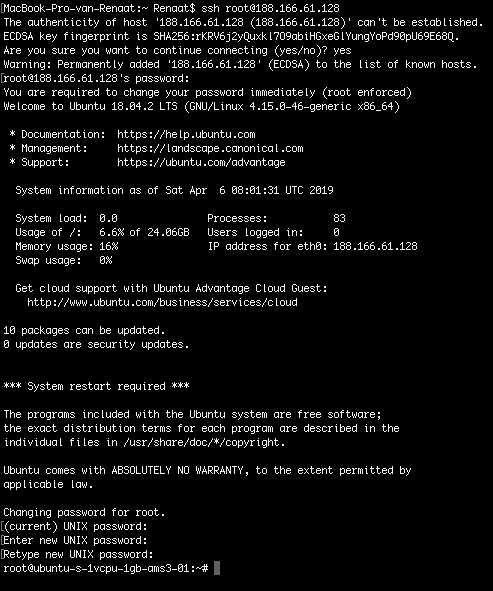
\includegraphics[scale=0.7]{OpzettenServer1}
                \caption{Opzetten Server, stap 1} \label{OpzettenServer1}
            \end{figure}
            
            SSH staat voor secure shell en is een software protocol dat voor een veilige verbinding (tunnel) zorgt tussen de client en de server. Het wordt gebruikt voor het configureren van een server, het beheren van netwerken en operating systems. Alle gegevens dat tussen beiden worden uitgevoerd zijn geëncrypteerd waardoor het moeilijker wordt voor hackers om de data te bemachtigen.
            
            Een server die gebruik maakt van SSH wordt ook wel een sshd server genoemd. Eens ingelogd op de sshd server moeten er enkele zaken aangepast worden aan de ssh configuratie in de file '/etc/ssh/sshd\_config'. Omdat we hier via de root gebruiker werken moet de property PermitRootLogin op yes staan. Dit zorgt ervoor dat de root gebruiker kan inloggen.
            StrictMode moet ook op yes staan, zo kan er niemand inloggen als de authenticatie documenten leesbaar zijn voor iedereen. Dit voor het beveiligen van configuratie documenten. Deze configuratie kan u zien in figuur\ref{OpzettenServer2} hier onder.
            
            \begin{figure}
                \centering
                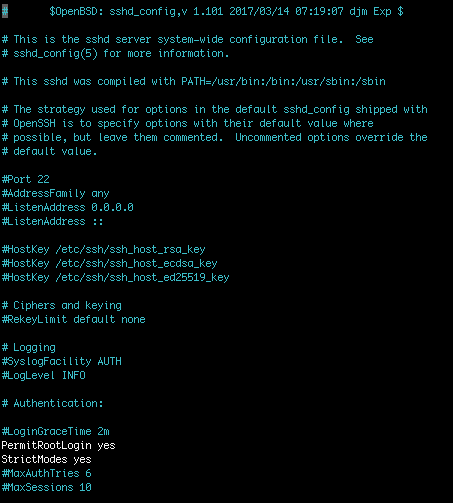
\includegraphics[scale=0.75]{OpzettenServer2}
                \caption{Opzetten Server, stap 2} \label{OpzettenServer2}
            \end{figure}
            
            De default manier om in te loggen via ssh is via een account en een paswoord, maar het is ook mogelijk om het account en het paswoord te vervangen door een private en een public key. Dit principe noemt key-based authentication en wordt vooral tijdens development en in scripts gebruikt of voor single sign-on. SSH genereert een private en een public key op de client wanneer deze stap wordt geconfigureerd. De private key moet veilig bewaard worden op de client computer. De public key moet doorgegeven worden aan de remote server. Wanneer de client wil inloggen op de server voert hij een request uit. De server maakt via zijn public key een bericht en stuurt dit als response door naar de client. De client leest het bericht aan de hand van zijn private key en stuurt dan een aangepaste response terug naar de remote server. De server valideert deze response. Bij een geldige private key zal er een goede response verstuurd worden, bij een ongeldige private key een foute response.
            In deze thesis gaat men ervan uit dat de client computer een ssh key heeft die gebruikt kan worden. Zoals u in figuur\ref{OpzettenServer3} kan zien heeft de client die gebruikt werd tijdens het schrijven van deze thesis enkel lees- en schrijfrechten voor de file 'id\_rsa', dit om het als secret te bewaren.
            De 'id\_rsa.pub' is de publieke key van de client die op de server moet komen om zo de ssh validatie te voorzien, dit wordt ook wel een ssh session genoemd. Eens de ssh session geconfigureerd is zal het niet nodig zijn om via een paswoord in te loggen op de remote server via deze client.
            In figuur\ref{OpzettenServer4} in de bijlagen is te zien hoe de ssh session wordt opgezet tussen de client en de remote server voor de root user.
            Voor deze thesis en om veiligheidsredenen is het beter om enkel via key-based authenticatie in te loggen en het paswoord uit te sluiten.
            In figuur\ref{OpzettenServer5} is te zien welke aanpassingen in de sshd\_config file van de sshd server moeten gebeuren om het niet meer mogelijk te maken om in te loggen via een paswoord. PasswordAuthentication en ChallengeResponseAuthentication moeten naar no verandert worden. PubKeyAuthentication moet naar yes verandert worden.
            Nu moet de 'sshd\_config' file opgeslagen worden (\^x + y + enter) en de ssh daemon herstart worden door het commando 'sudo systemctl restart ssh' in te geven.
            
            \begin{figure}
                \centering
                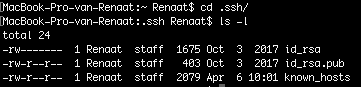
\includegraphics{OpzettenServer3}
                \caption{Opzetten Server, stap 3} \label{OpzettenServer3}
            \end{figure}
        
            \begin{figure}
                \centering
                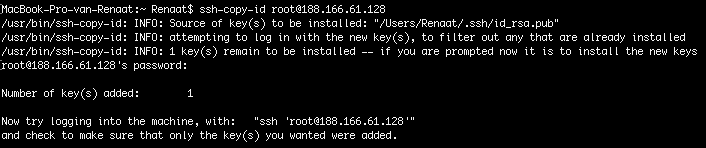
\includegraphics[scale=0.65]{OpzettenServer4}
                \caption{Opzetten Server, stap 4} \label{OpzettenServer4}
            \end{figure}
        
            \begin{figure}
                \centering
                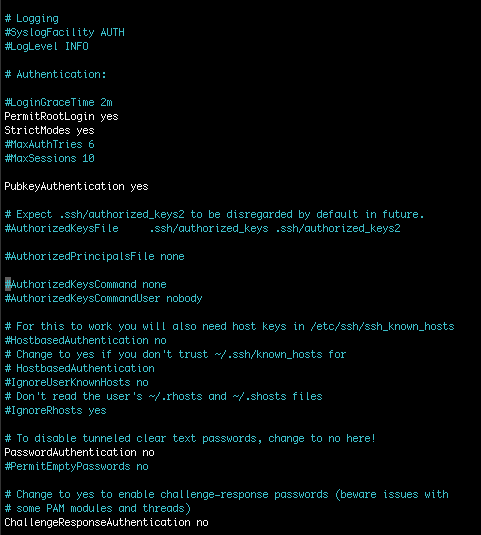
\includegraphics[scale=0.75]{OpzettenServer5}
                \caption{Opzetten Server, stap 5} \label{OpzettenServer5}
            \end{figure}
            
            Om de remote server nog meer te beschermen tegen cyber aanvallen is het nodig om een firewall op te zetten. In deze voorbeeldapplicatie maken we gebruik van de UFW Firewall. Dis staat voor Uncomplicated Firewall en is een gebruiksvriendelijke tool dat helpt om de iptables onder controle te houden om zo te zorgen dat bepaalde services toegelaten worden tot onze server.
            In Linux maken ze gebruik van het protocol SSH via de service OpenSSH, deze heeft ook een profiel bij UFW.
            In Figuur\ref{OpzettenServer6} in de bijlagen is te zien hoe de firewall de SSH service toelaat. Het is enkel mogelijk om de server te bereiken via deze service. Later worden er uiteraard meerdere services toegelaten.
            
            \begin{figure}
                \centering
                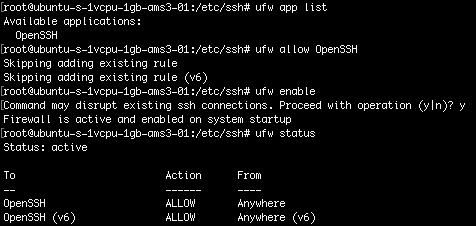
\includegraphics[scale=0.9]{OpzettenServer6}
                \caption{Opzetten Server, stap 6} \label{OpzettenServer6}
            \end{figure}
            
            Nu alle stappen voor de configuratie van de server gedaan zijn is het zeer makkelijk om in te loggen op de server.
            Het is hetzelfde als de eerste keer, maar nu vraagt de server niet meer naar een paswoord, maar gebruikt hij de ssh-key. Het is voldoende om 
            'ssh root@188.166.61.128' te typen om in te loggen.
            Als je wil uitloggen is het nodig om in de command line van de server exit te typen.
    
        \subsection{Database}
        \label{subsec:database}
        Binnen SAP wordt een HANA database aangeraden om te gebruiken. Momenteel is versie 2.0 van SAP HANA op de markt en deze versie biedt tal van extra mogelijkheden ten opzichte van de vorige versie. SAP HANA wordt zeer goed ondersteund door de andere programma's binnen SAP en wordt daarom ook wel veel gebruikt.
        Voor de database maken we gebruik van een Multi-Target Application Project, dit is een template die SAP ons geeft en is een goede uitvalsbasis om te gebruiken in de voorbeeldapplicatie.
        Zoals eerder al aangegeven is een Source Code Repository van groot belang voor een CI/CD pipeline en development in het algemeen.
        
            \paragraph{Source Control \& Databank module}
            In figuur\ref{SourceControl1} kan u waarnemen hoe een repository gemaakt wordt in Bitbucket.
            Eens de repository aangemaakt is heb je het webadres nodig om de clone te maken op je lokale machine.
            
            \begin{figure}
                \centering
                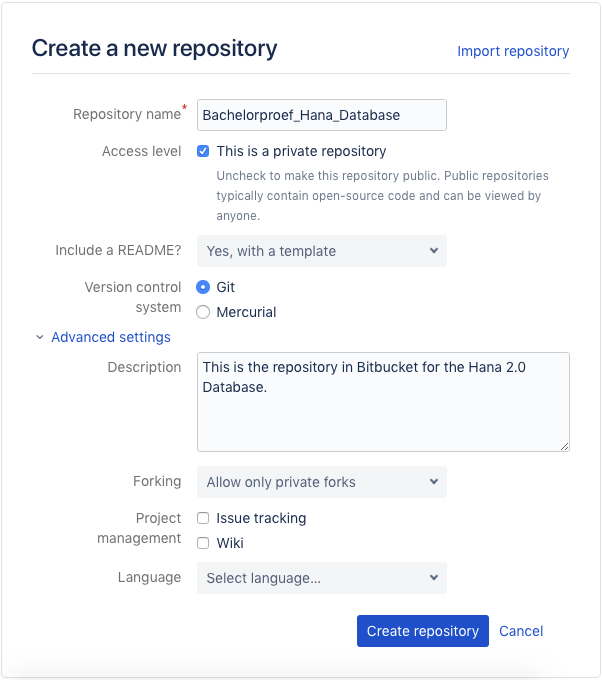
\includegraphics[scale=0.5]{SourceControl1}
                \caption{Source Control, stap 1} \label{SourceControl1}
            \end{figure}
            
            De volgende stap is het project aanmaken. In de Web IDE voor HANA development is het belangrijk om eerst enkele instellingen aan te passen.
            Alle nodige features die nodig zijn kan u terug vinden in figuur\ref{HANA1}. Nu is het ook belangrijk om je Git account te connecteren met de Web IDE door het Git email adres en Git username in te voeren in de Git Settings.
            Zoals eerder vermeld maken we het project aan de hand van het Multi-Target Application Project template. na de creatie van het project is het nodig om een build uit te voeren (figuur\ref{HANA2}).
            Om het project aan het account op Bitbucket te linken klikt u op het project met de rechter muisknop, gaat u naar 'Git' en dan 'Initialize Local Repository' (figuur\ref{HANA3}).
            Nu linken we de gemaakte repository aan het project door via rechter muisklik op het project op Git en dan Set Remote te klikken. Hier moet je de gekopieerde Bitbucket link plakken in het veld voor URL. Na het ingeven van het juiste wachtwoord, is het nodig om op 'OK' te klikken wanneer het 'Changes Fetched' window opent. Deze stappen zijn te volgen in figuren \ref{HANA4} en \ref{HANA5}.
            Na deze stap is het project gelinkt met de repository op Bitbucket. Het maken van het project heeft voor changes gezorgd in de repository, deze moeten eerst gecommit en gepusht worden. In figuur\ref{HANA6} is te zien wat er allemaal moet gebeuren om een commit en push te doen naar de repository.
    
            \begin{figure}
                \centering
                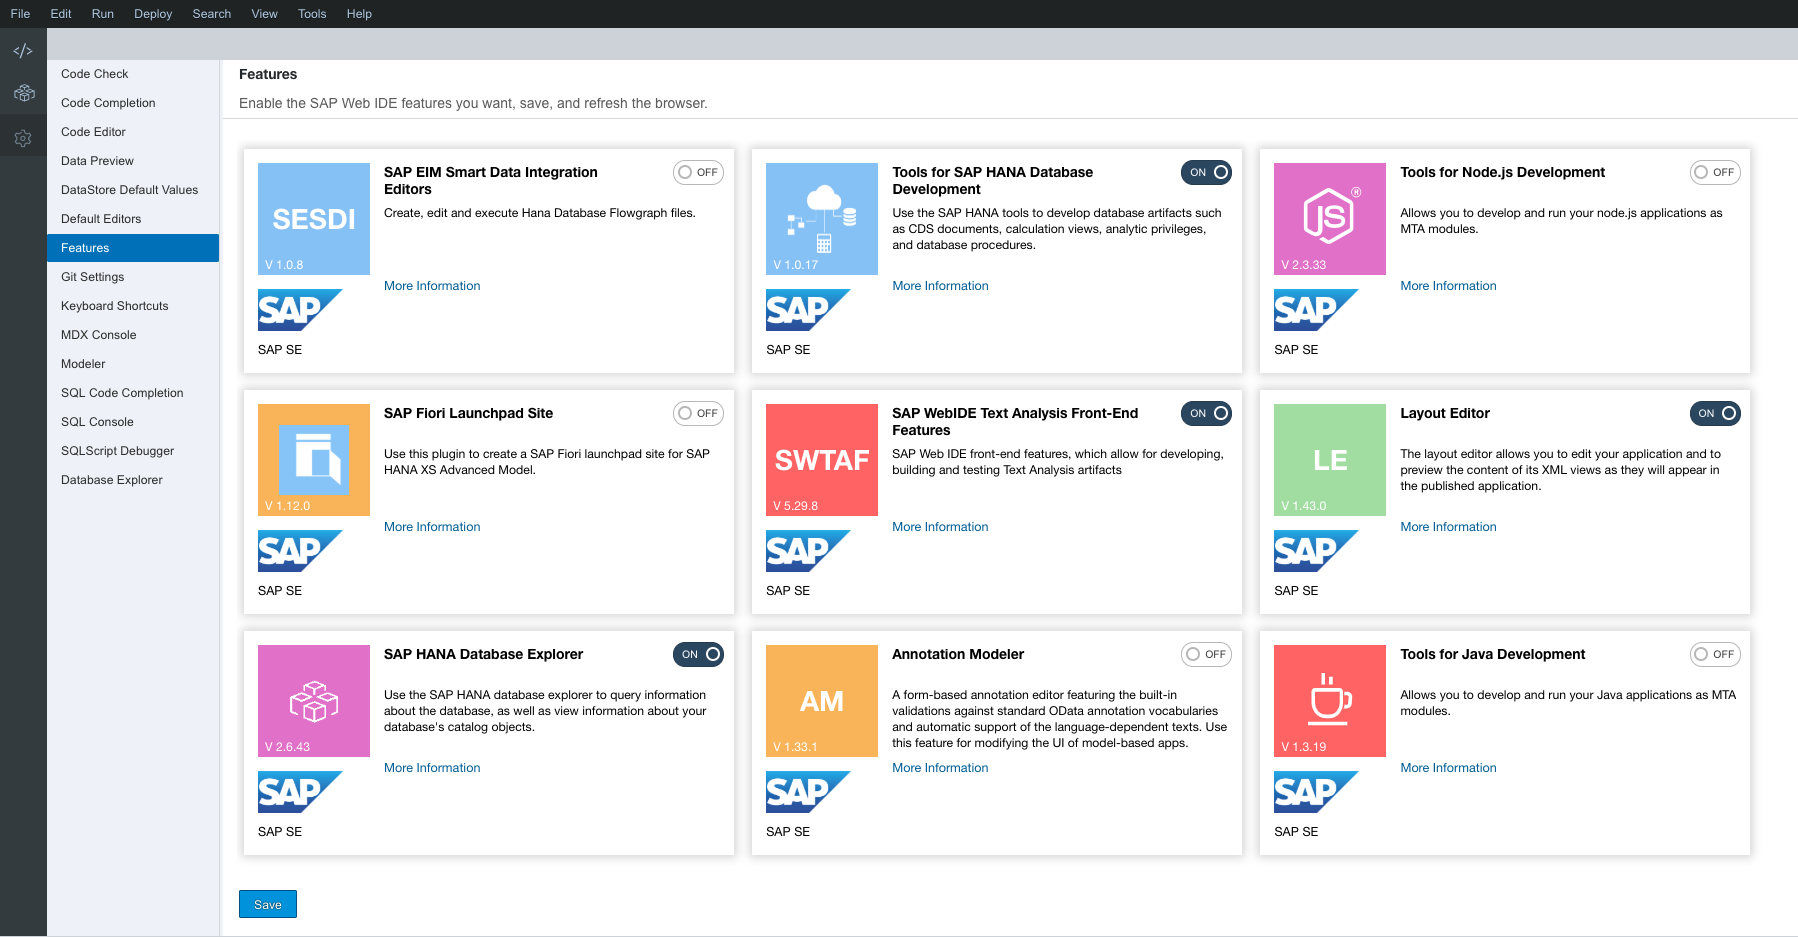
\includegraphics[scale=0.25]{HANA1}
                \caption{Opzetten HANA, stap 1} \label{HANA1}
            \end{figure}
        
            \begin{figure}	
                \centering
                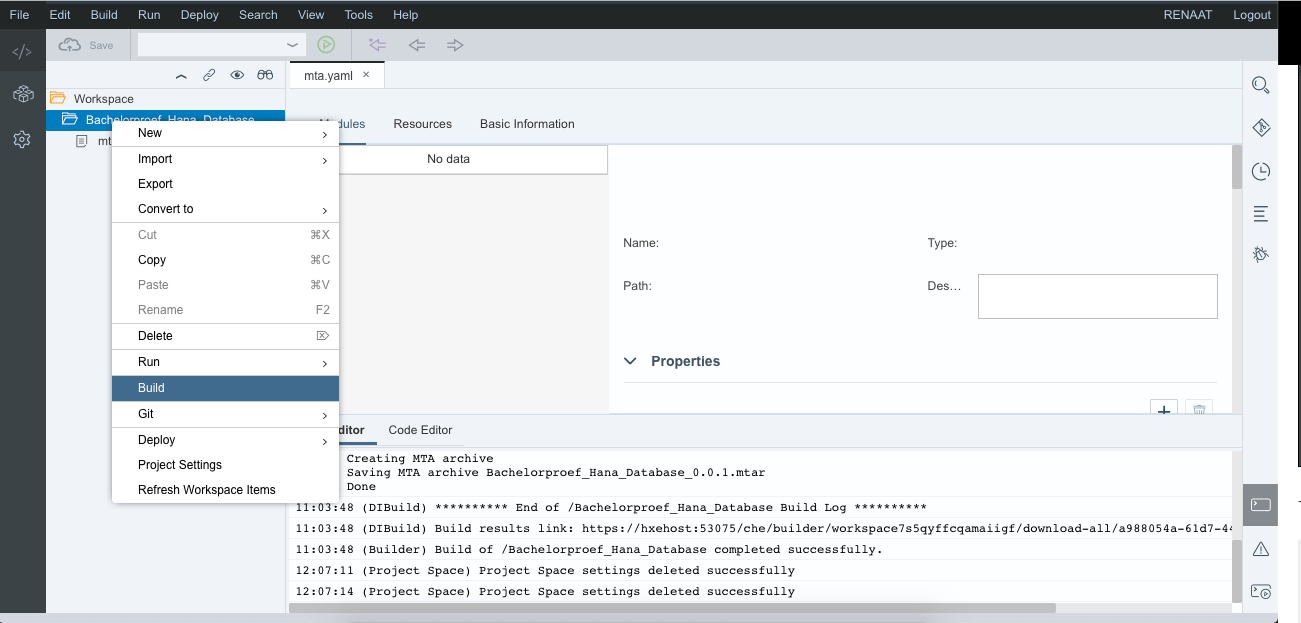
\includegraphics[scale=0.35]{HANA2}
                \caption{Opzetten HANA, stap 2} \label{HANA2}
            \end{figure}
            
            \begin{figure}	
                \centering
                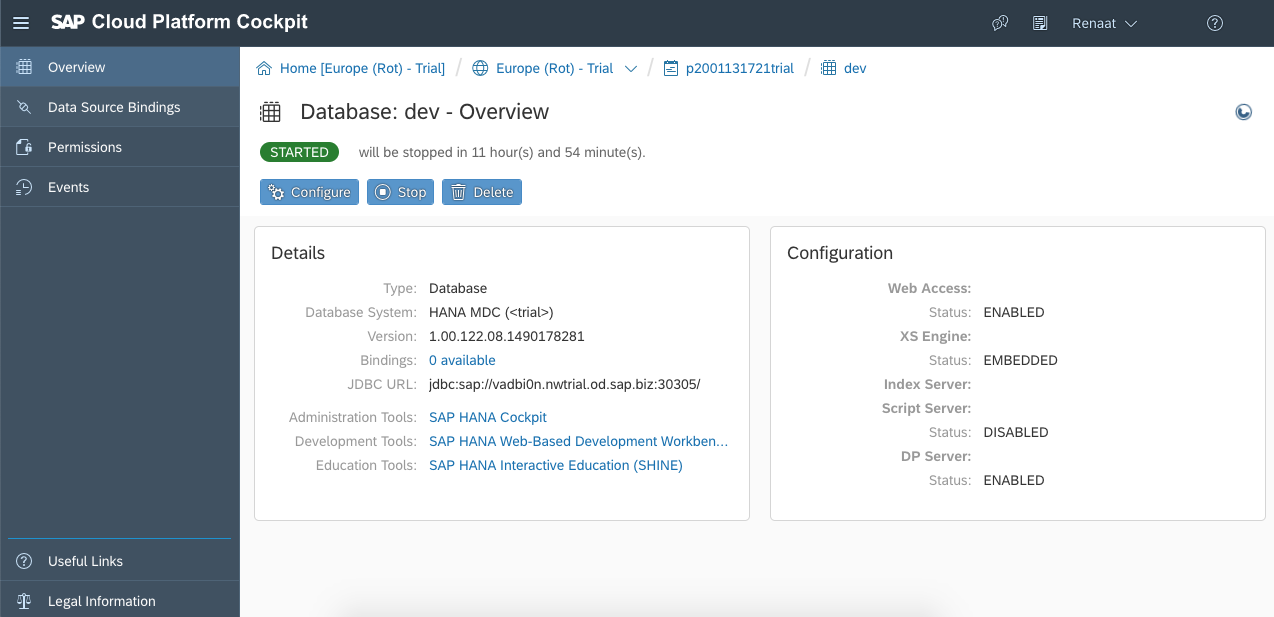
\includegraphics[scale=0.35]{HANA3}
                \caption{Opzetten HANA, stap 3} \label{HANA3}
            \end{figure}
        
            \begin{figure}	
                \centering
                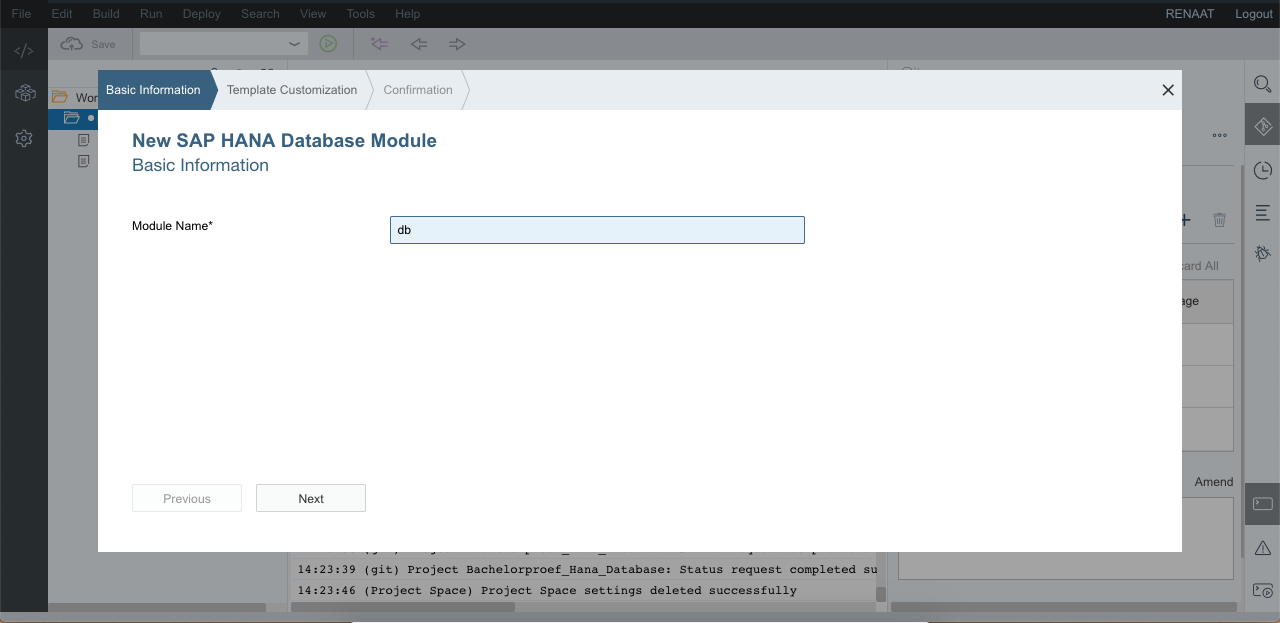
\includegraphics[scale=0.35]{HANA4}
                \caption{Opzetten HANA, stap 4} \label{HANA4}
            \end{figure}
        
            \begin{figure}	
                \centering
                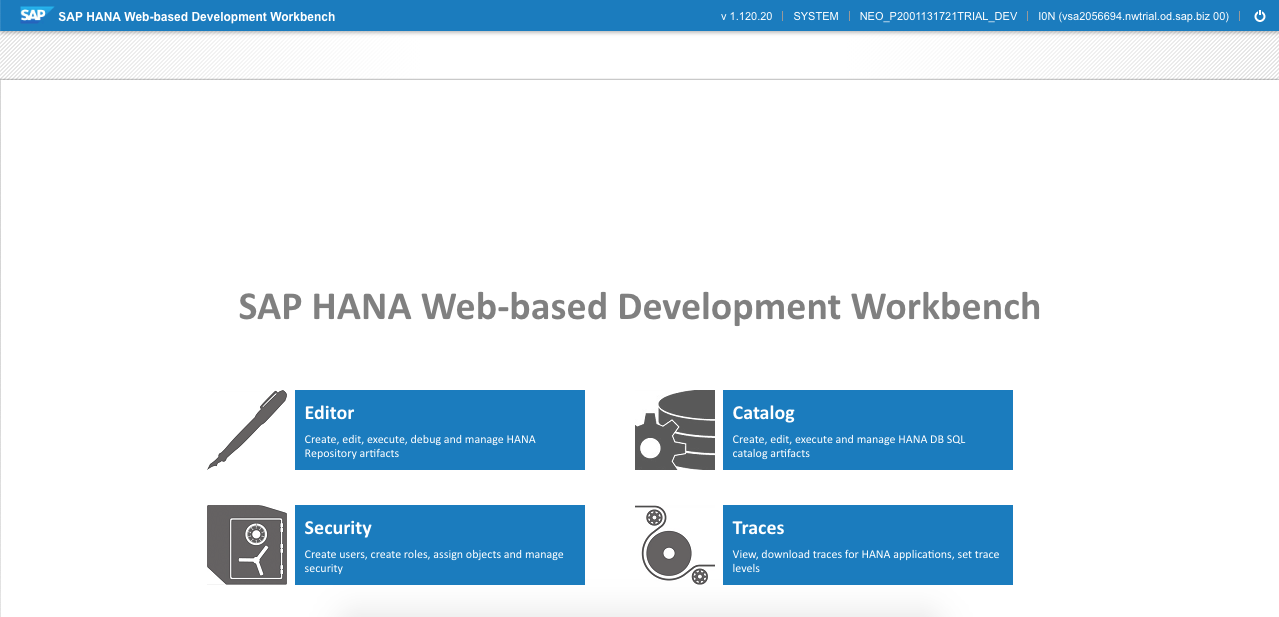
\includegraphics[scale=0.35]{HANA5}
                \caption{Opzetten HANA, stap 5} \label{HANA5}
            \end{figure}
        
            \begin{figure}	
                \centering
                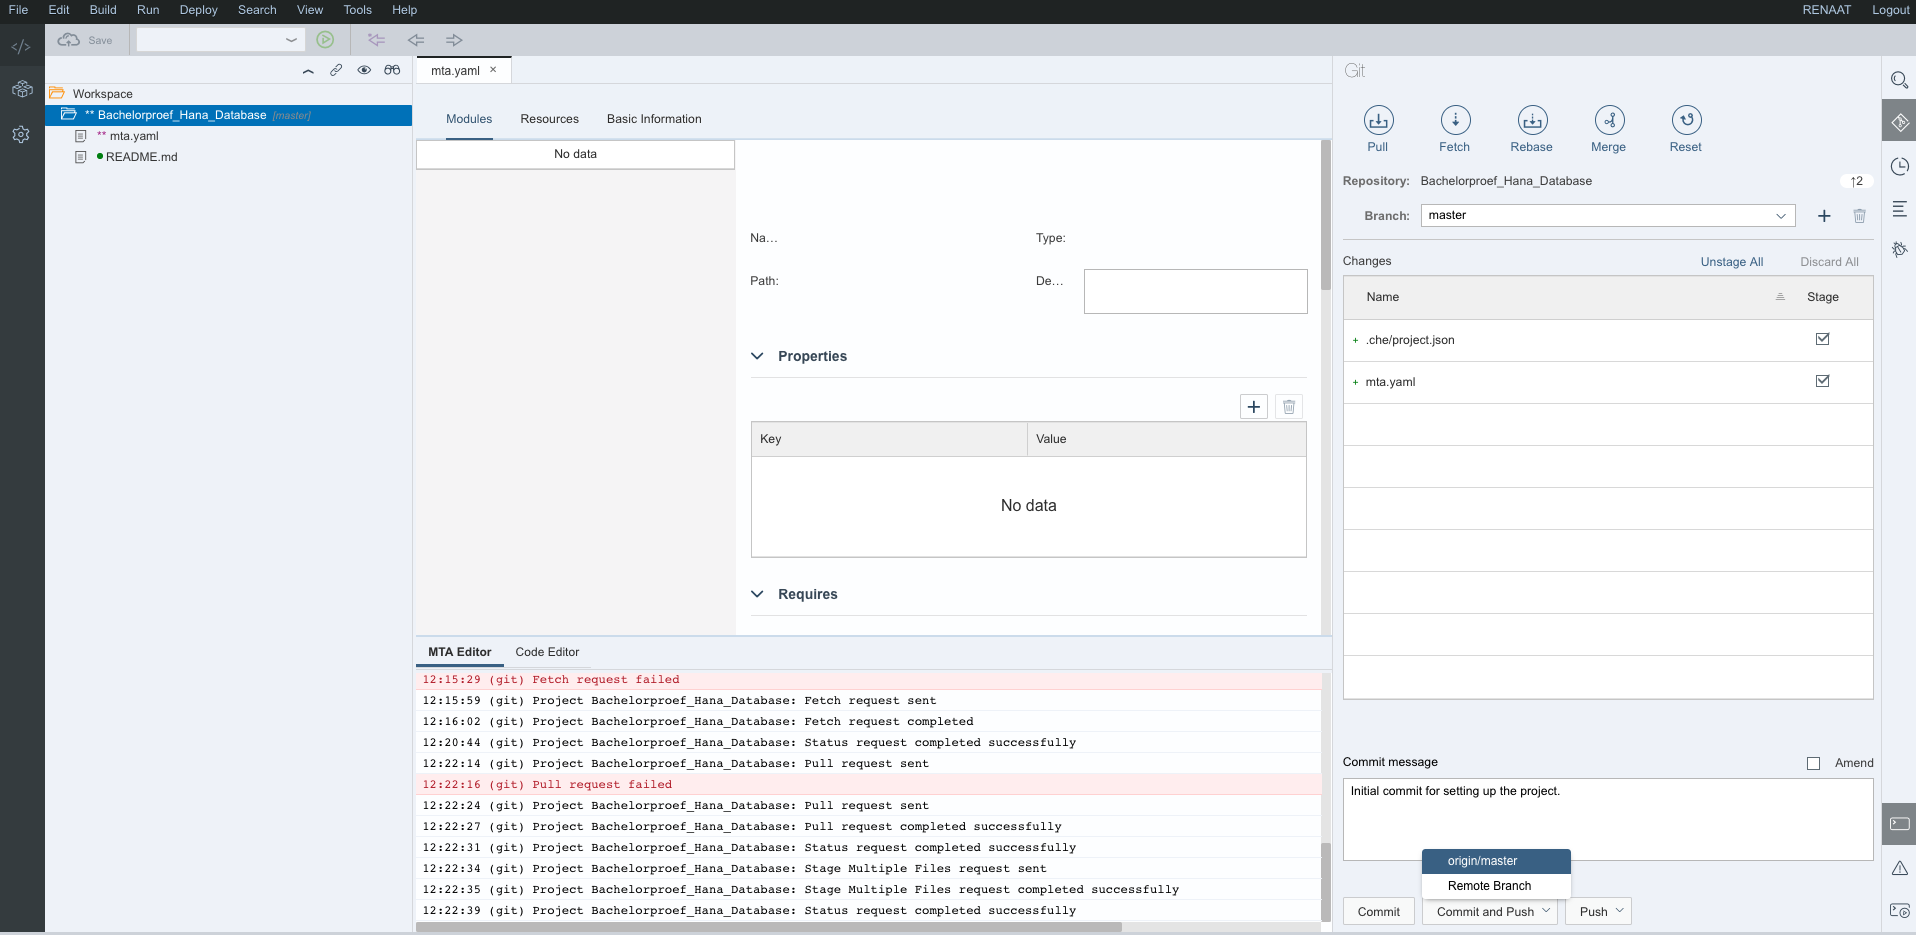
\includegraphics[scale=0.2]{HANA6}
                \caption{Opzetten HANA, stap 6} \label{HANA6}
            \end{figure}
            
            Een realistische opstelling van een CI/CD voorbeeldapplicatie start bijna nooit vanaf nul, het bouwt meestal voort op bestaande, geschreven software.
            Daarom zal er in deze voorbeeldapplicatie manueel een basis gelegd worden, zo kan er aan de hand van een build scheduler voortgebouwd worden op deze geschreven software.
            De bescheiden database waar we naartoe willen gaan bestaat uit twee entiteiten: een Artiest en een Album. Een artiest kan meerdere albums hebben, maar een album kan maar tot één artiest behoren. De entiteit Artiest heeft volgende properties: ID, Naam, JaarVanOorsprong en Stad. Album heeft ID, Naam, Beschrijving, Genre, Jaar en Studio als properties. Als basis maken we de entiteit Artiest enkel met ID, Naam en JaarVanOorsprong. De rest zal later toegevoegd worden aan de hand van de pipeline.
            Eerst maken we een HANA Database Module zoals in figuren \ref{HANA7}, \ref{HANA8} en \ref{HANA9} te zien zijn. Daarna wordt een HDB CDS Artifact gemaakt. Dit is een Core Data Services document dat defenities bevat om objecten te creëeren in de database. Hoe de Artiest gedefinieerd wordt kan u zien in figuren \ref{HANA10}, \ref{HANA11}, \ref{HANA12} en \ref{HANA13}.
            Nu alle gegevens ingevoerd zijn, moeten we de database effectief aanmaken. In de meest linkse tab is er een knop 'Database Explorer' genaamd. Als je daar op klikt zie je een lege kolom verschijnen. Je moet op het +-teken klikken om een database aan te maken. Kies uit de lijst de optie met jouw naam en geef een realistische naam bij het veld 'How to Show in Display'. Laat de rest van de setting zoals ze zijn.
            Dan is het de bedoeling om de gegevens die we hierboven hebben ingevoerd in de net aangemaakte database komen. Dit doe je door terug te gaan naar de 'Development' omgeving (in meest linkse tab), daar met de rechter muisknop op 'data.hdbcds' file te klikken en voor de optie 'Build Selected Files' te kiezen. De stappen kan je volgen in figuren \ref{HANA14} en \ref{HANA15}.
            Er moet natuurlijk ook data in de database zitten om deze te gebruiken in de SAPUI5 applicatie. Een manier om dit te doen is via het uploaden van csv-bestanden waar de data gescheiden is door een komma. Om dit te kunnen uploaden moet er een nieuwe file aangemaakt worden in de data map van de db-module, 'load.hdbtabledata' genaamd. De inhoud kan u ook vinden in figuur \ref{HANA16}.
            In dit voorbeeld wordt er gebruik gemaakt van een csv-bestand dat nog aangemaakt moet worden. De inhoud van dit bestand is te zien in figuur \ref{HANA17}. Deze gemaakte file moet geïmporteerd worden in de map data van de db-module zoals te zien is in figuur \ref{HANA18}. Om dit te controleren open je best de file nog eens, de inhoud moet overeenkomen met wat in figuur \ref{HANA19} te zien is. Eens deze stappen volbracht zijn is het tijd om de module te builden (figuur \ref{HANA20}). Om te kijken of de data er juist inzit moet je terug gaan naar de 'Database Explorer' en daar de map 'tables' openen. Links vanonder verschijnt een venster met de verschillende tabellen, hier in dit voorbeeld is er maar één, dus we kunnen niet verkeerd zijn. Er rest ons enkel nog op de juiste tabel te klikken met de rechter muisknop en dan op 'Generate SELECT statement' aan te klikken. Er opent zich een nieuwe file die moet uitgevoerd worden zoals in figuren \ref{HANA21}, \ref{HANA22} en \ref{HANA23} te zien zijn.
            Eens deze gegevens ingevoerd zijn moeten we alle veranderingen toevoegen aan de commit om dan te pushen naar de repository.
            
            
            \begin{figure}	
                \centering
                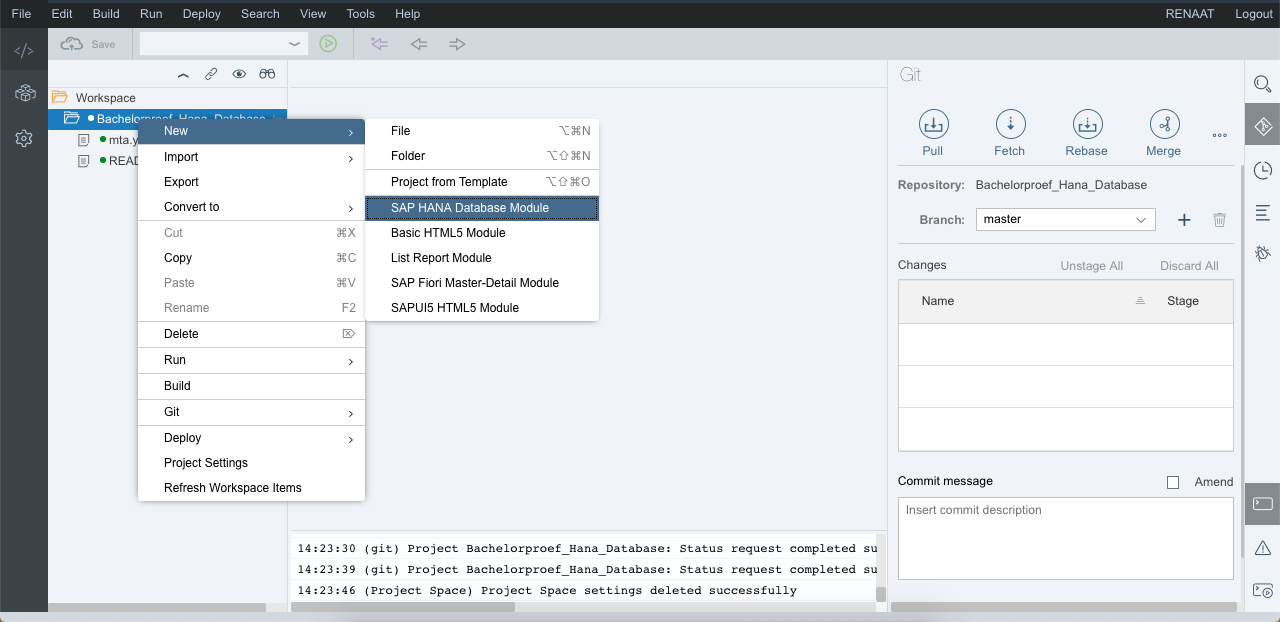
\includegraphics[scale=0.35]{HANA7}
                \caption{Opzetten HANA, stap 7} \label{HANA7}
            \end{figure}
            
            \begin{figure}	
                \centering
                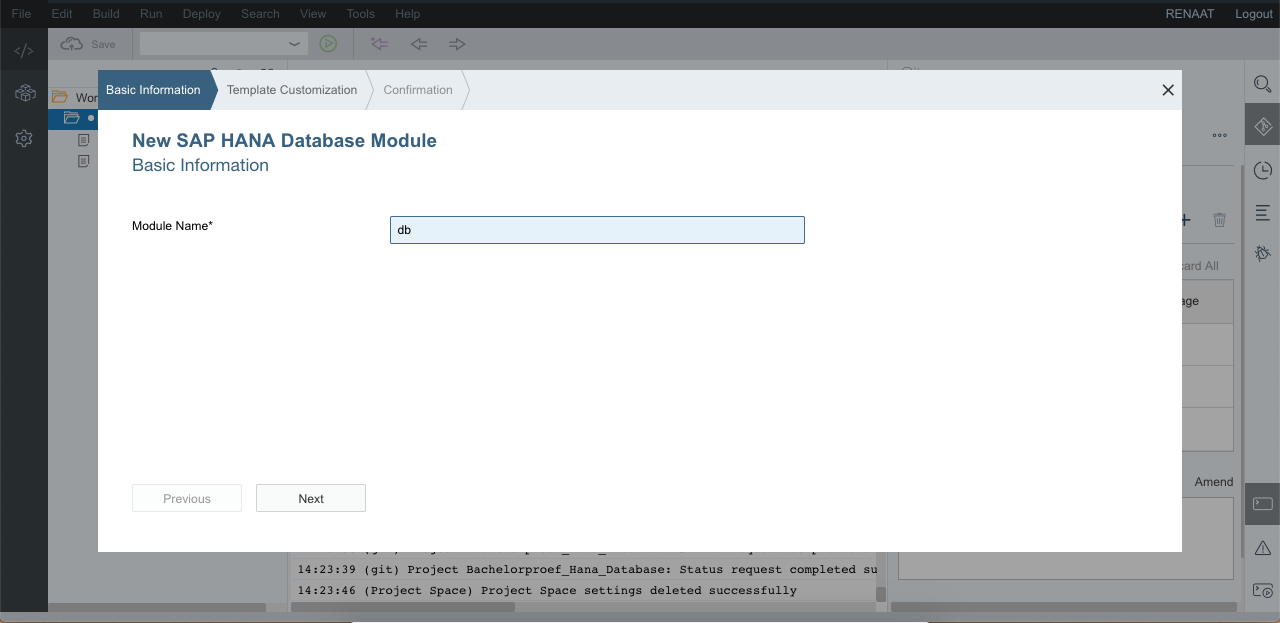
\includegraphics[scale=0.35]{HANA8}
                \caption{Opzetten HANA, stap 8} \label{HANA8}
            \end{figure}
            
            \begin{figure}	
                \centering
                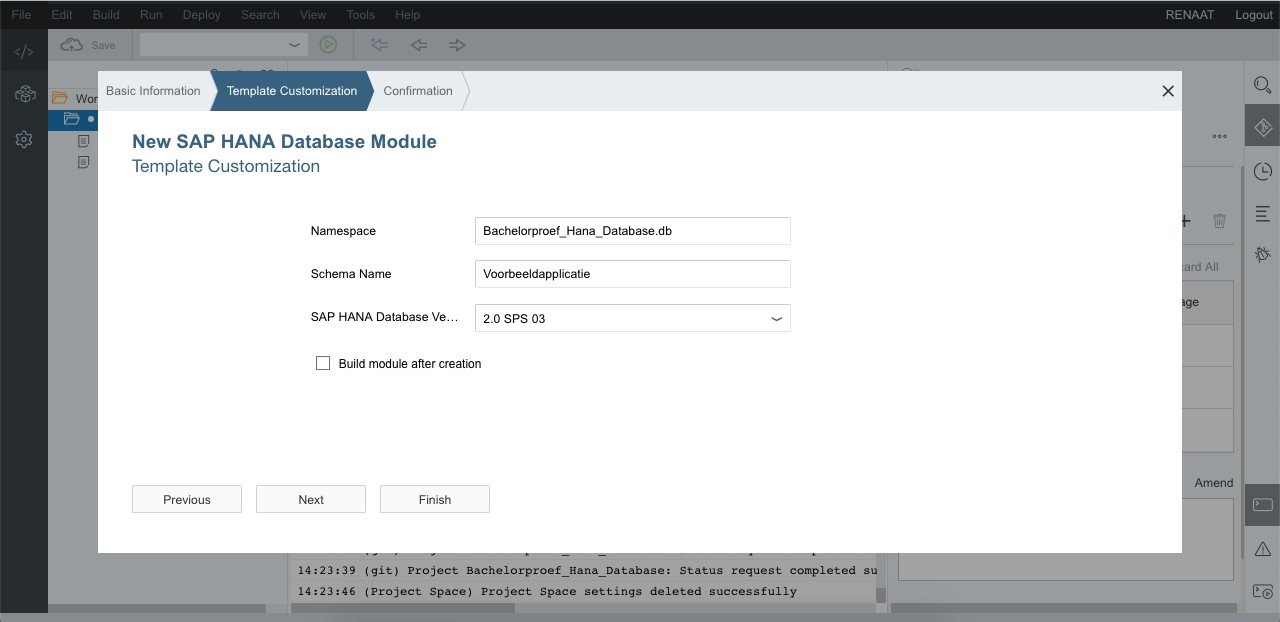
\includegraphics[scale=0.35]{HANA9}
                \caption{Opzetten HANA, stap 9} \label{HANA9}
            \end{figure}
            
            \begin{figure}	
                \centering
                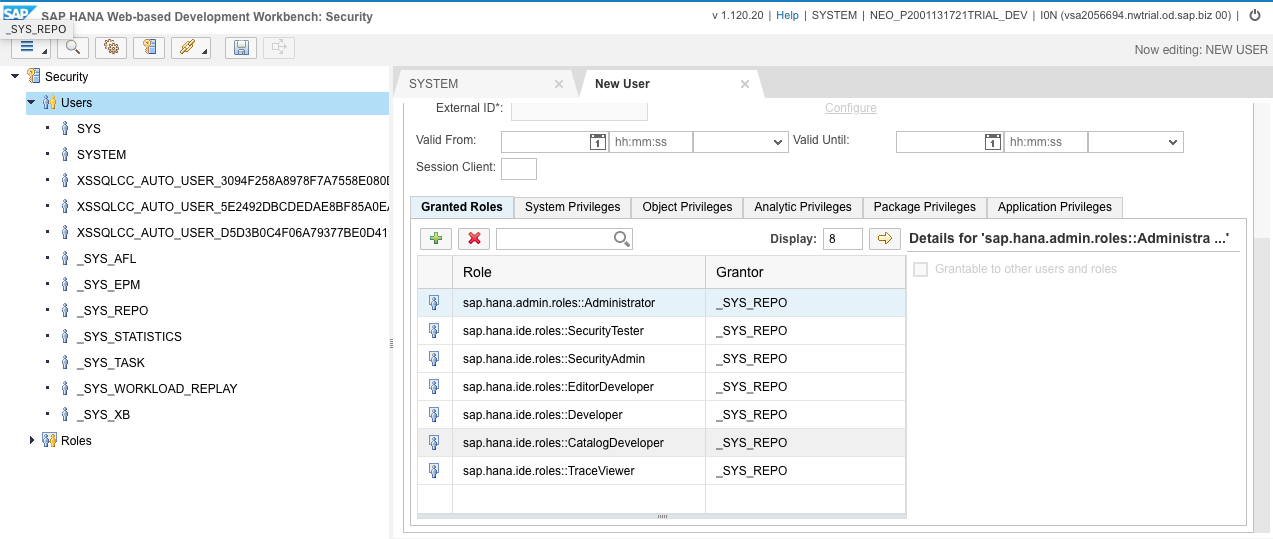
\includegraphics[scale=0.35]{HANA10}
                \caption{Opzetten HANA, stap 10} \label{HANA10}
            \end{figure}
            
            \begin{figure}	
                \centering
                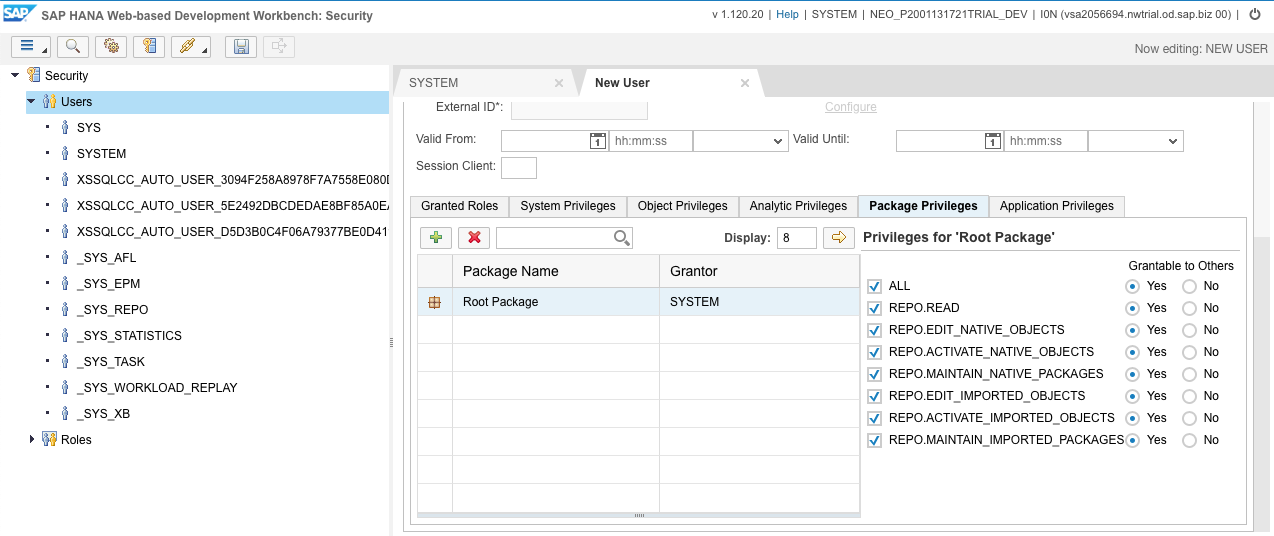
\includegraphics[scale=0.35]{HANA11}
                \caption{Opzetten HANA, stap 11} \label{HANA11}
            \end{figure}
            
            \begin{figure}	
                \centering
                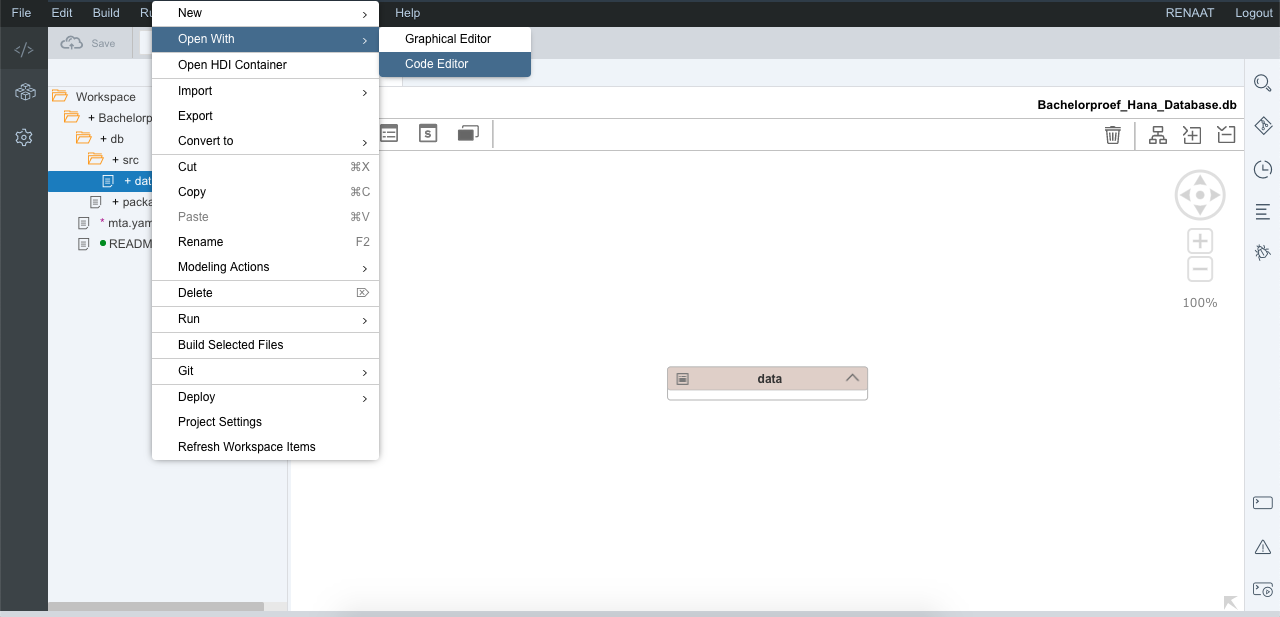
\includegraphics[scale=0.35]{HANA12}
                \caption{Opzetten HANA, stap 12} \label{HANA12}
            \end{figure}
        
            \begin{figure}	
                \centering
                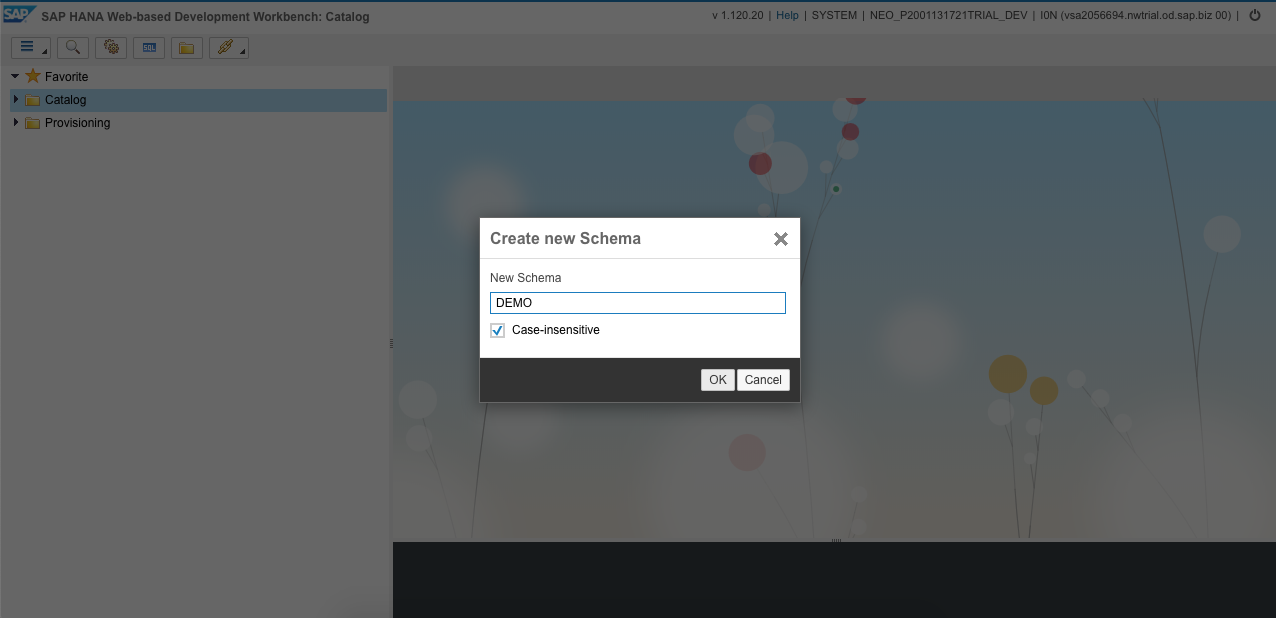
\includegraphics[scale=0.35]{HANA13}
                \caption{Opzetten HANA, stap 13} \label{HANA13}
            \end{figure}
            
            \begin{figure}	
                \centering
                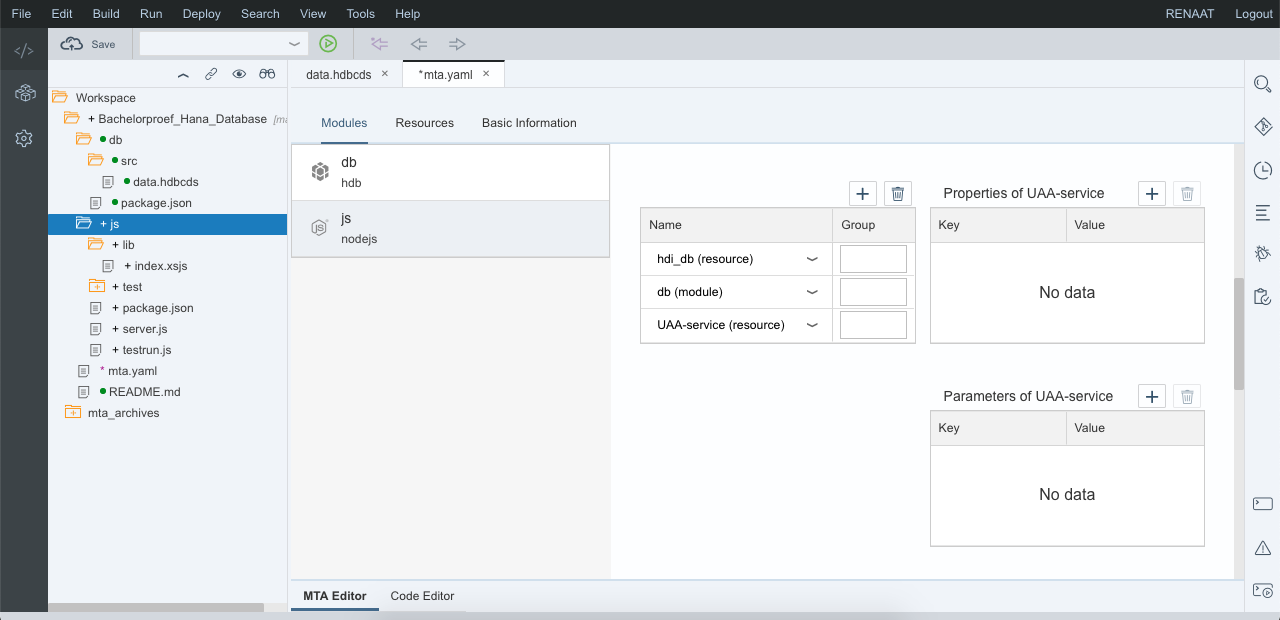
\includegraphics[scale=0.35]{HANA14}
                \caption{Opzetten HANA, stap 14} \label{HANA14}
            \end{figure}
            
            \begin{figure}	
                \centering
                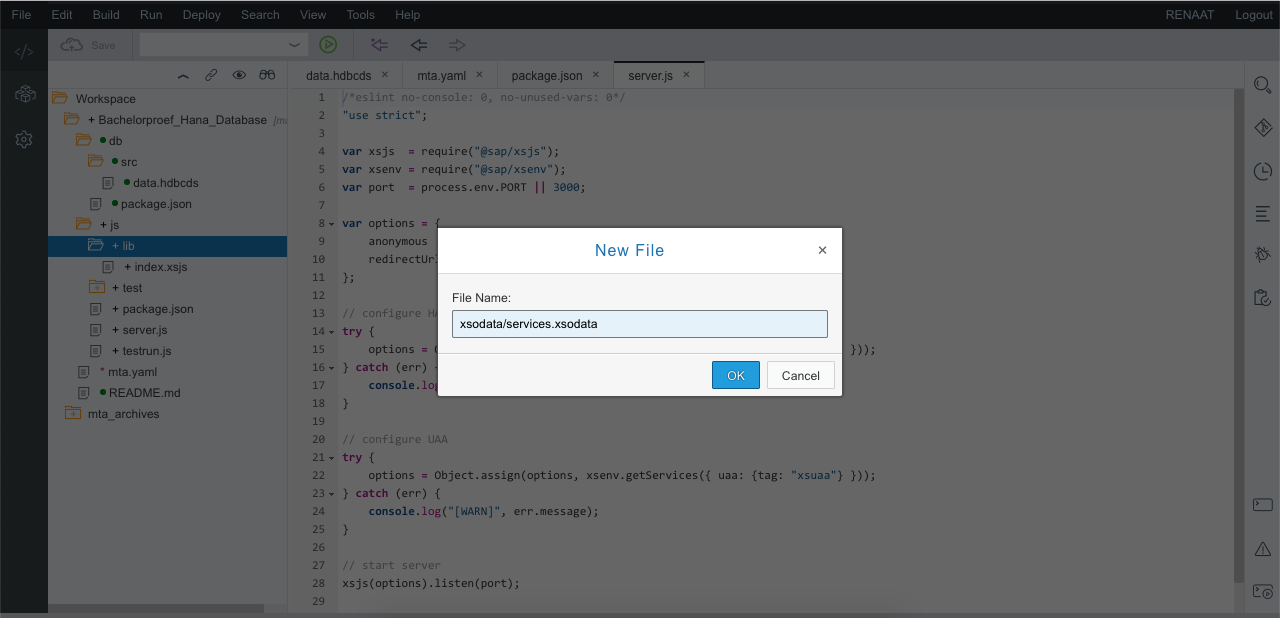
\includegraphics[scale=0.35]{HANA15}
                \caption{Opzetten HANA, stap 15} \label{HANA15}
            \end{figure}
        
            \begin{figure}	
                \centering
                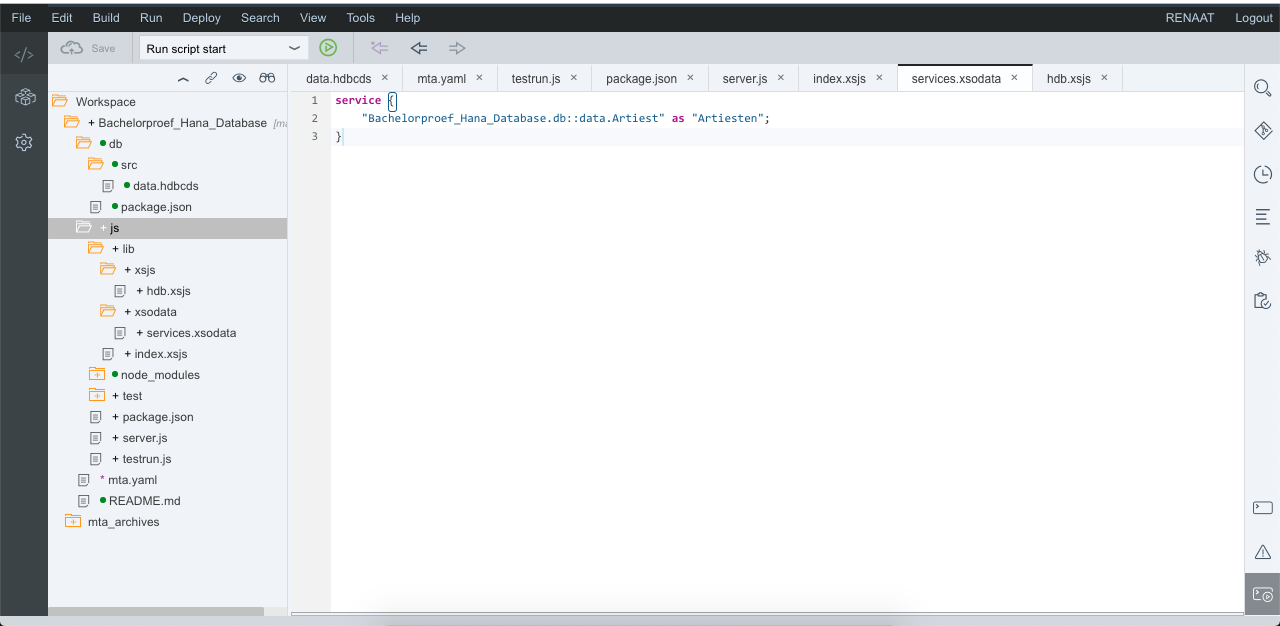
\includegraphics[scale=0.35]{HANA16}
                \caption{Opzetten HANA, stap 16} \label{HANA16}
            \end{figure}
            
            \begin{figure}	
                \centering
                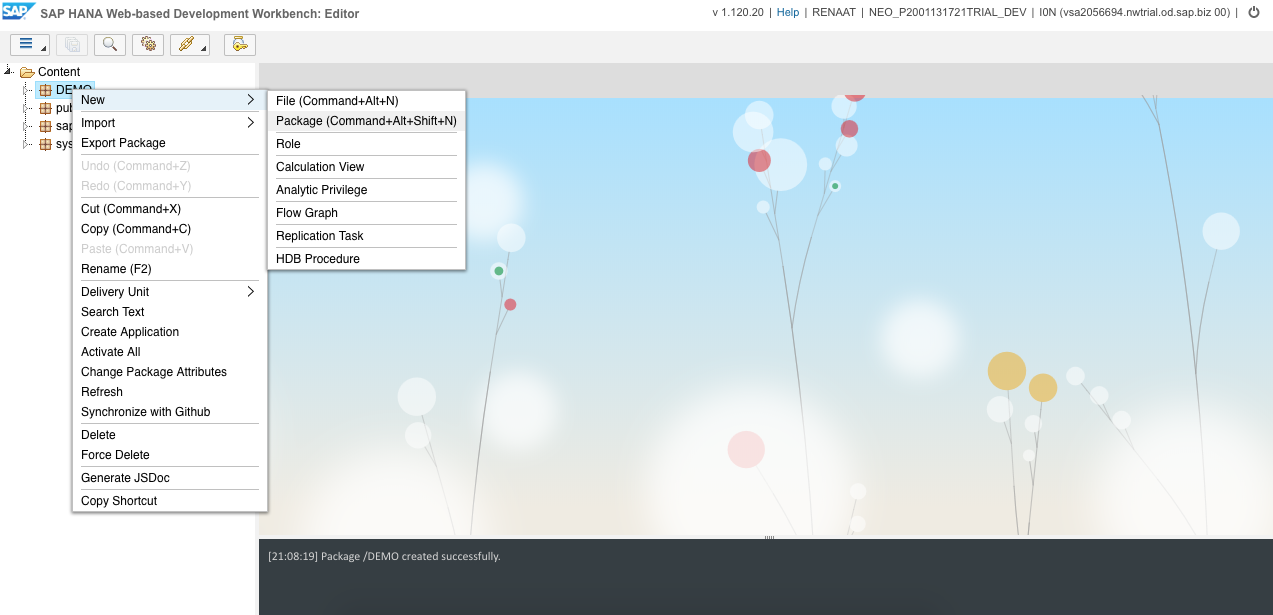
\includegraphics[scale=0.35]{HANA17}
                \caption{Opzetten HANA, stap 17} \label{HANA17}
            \end{figure}
        
            \begin{figure}	
                \centering
                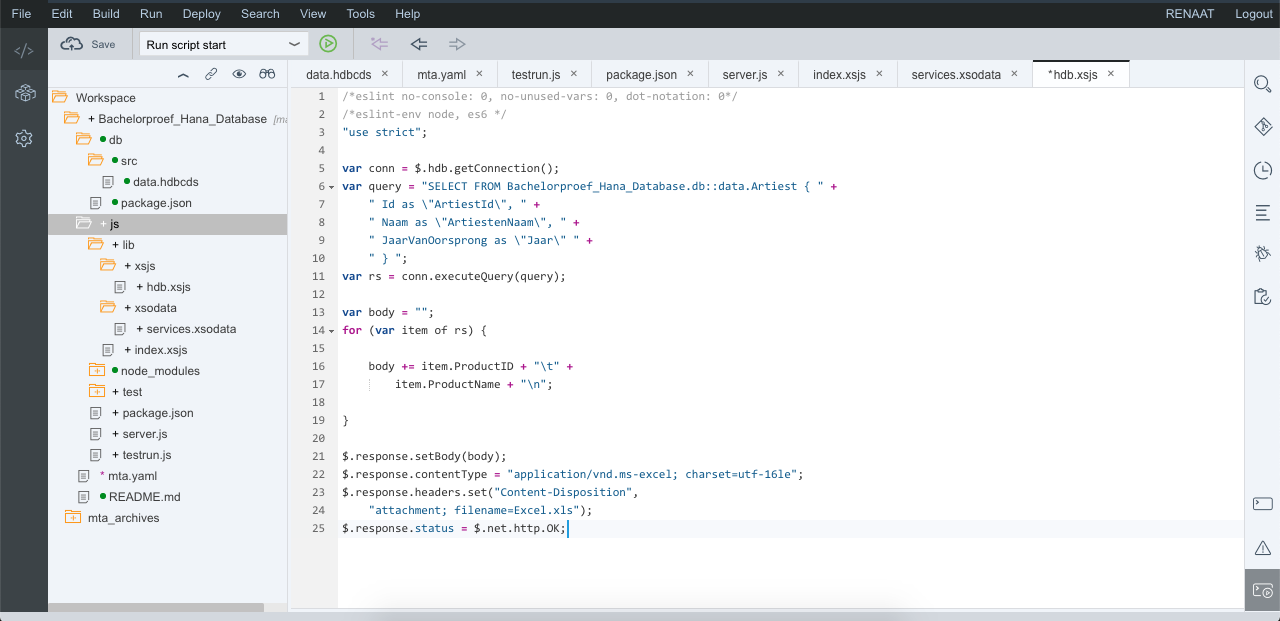
\includegraphics[scale=0.35]{HANA18}
                \caption{Opzetten HANA, stap 18} \label{HANA18}
            \end{figure}
            
            \begin{figure}	
                \centering
                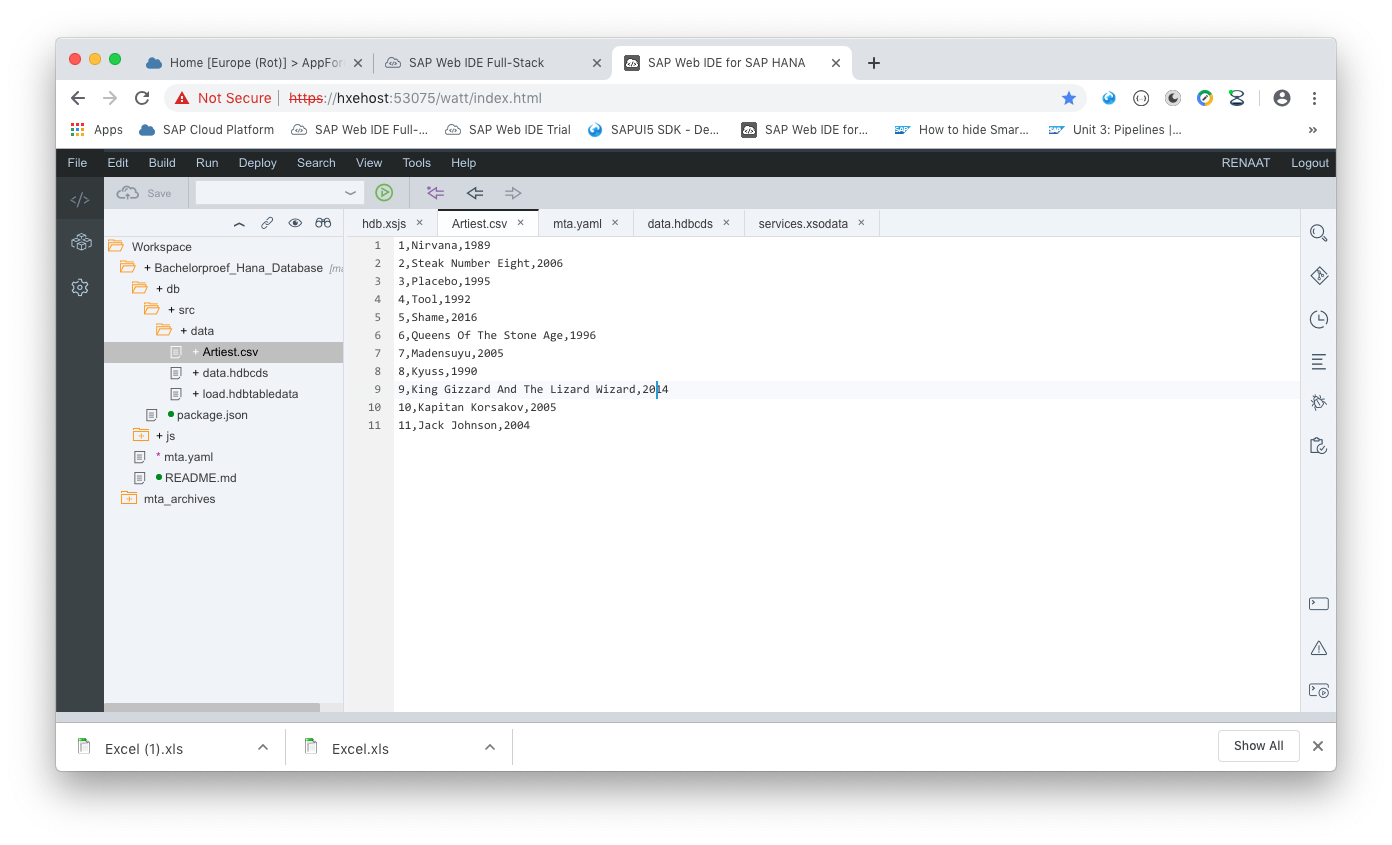
\includegraphics[scale=0.35]{HANA19}
                \caption{Opzetten HANA, stap 19} \label{HANA19}
            \end{figure}
        
            \begin{figure}	
                \centering
                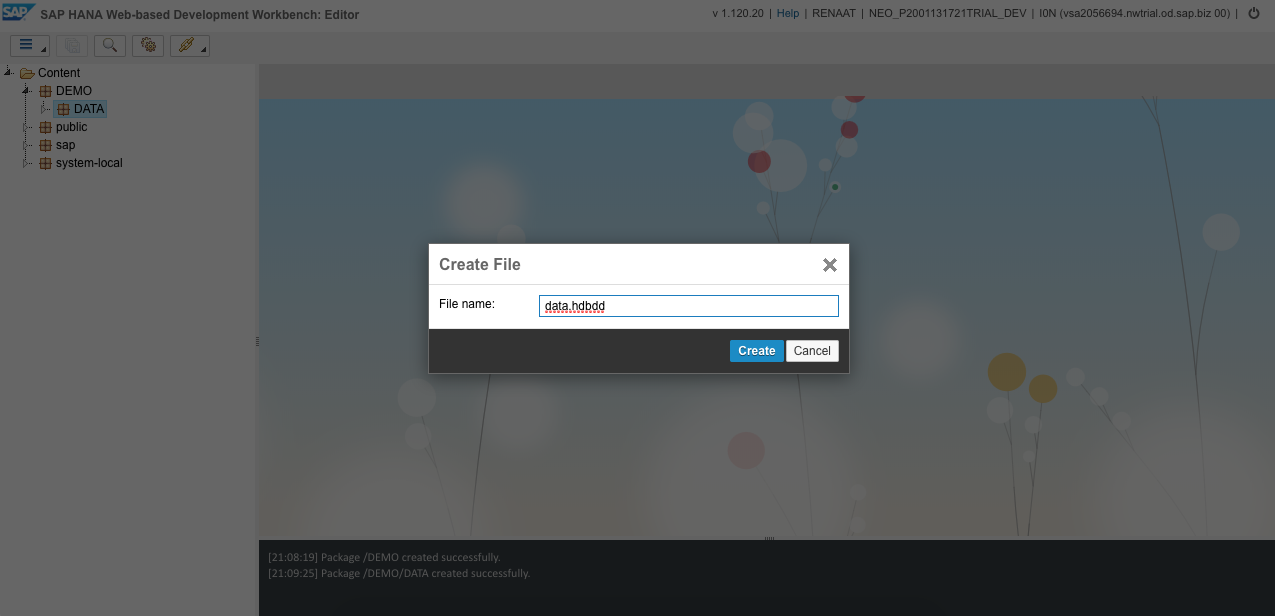
\includegraphics[scale=0.35]{HANA20}
                \caption{Opzetten HANA, stap 20} \label{HANA20}
            \end{figure}
            
            \begin{figure}	
                \centering
                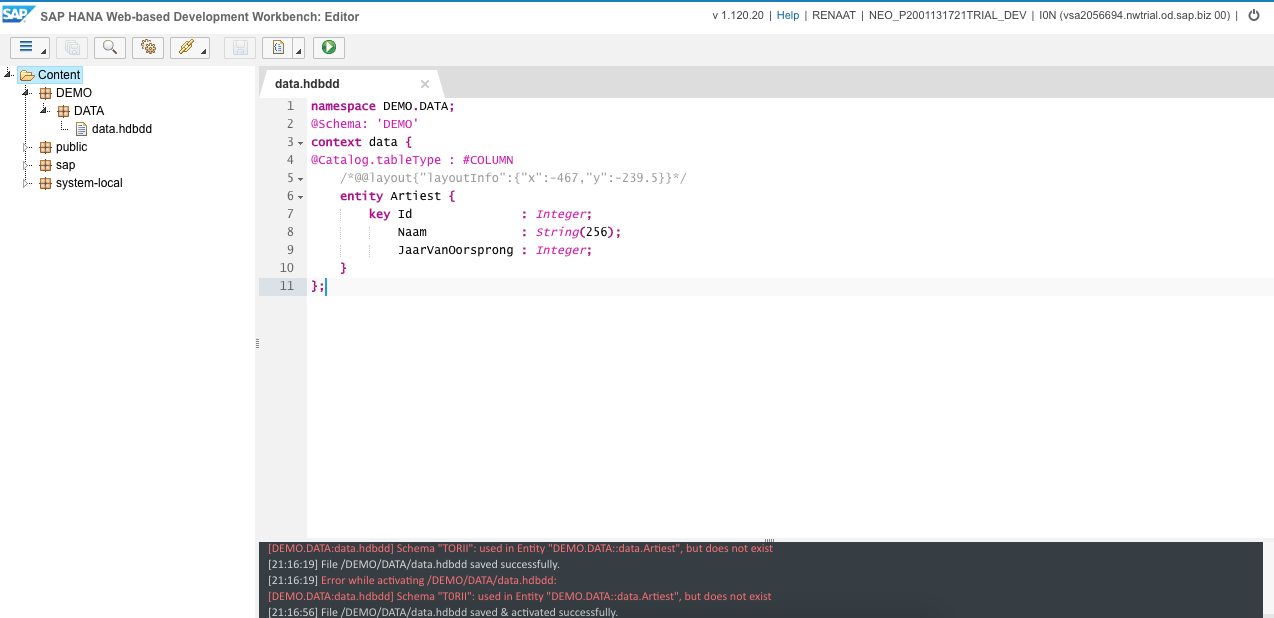
\includegraphics[scale=0.35]{HANA21}
                \caption{Opzetten HANA, stap 21} \label{HANA21}
            \end{figure}
        
            \begin{figure}	
                \centering
                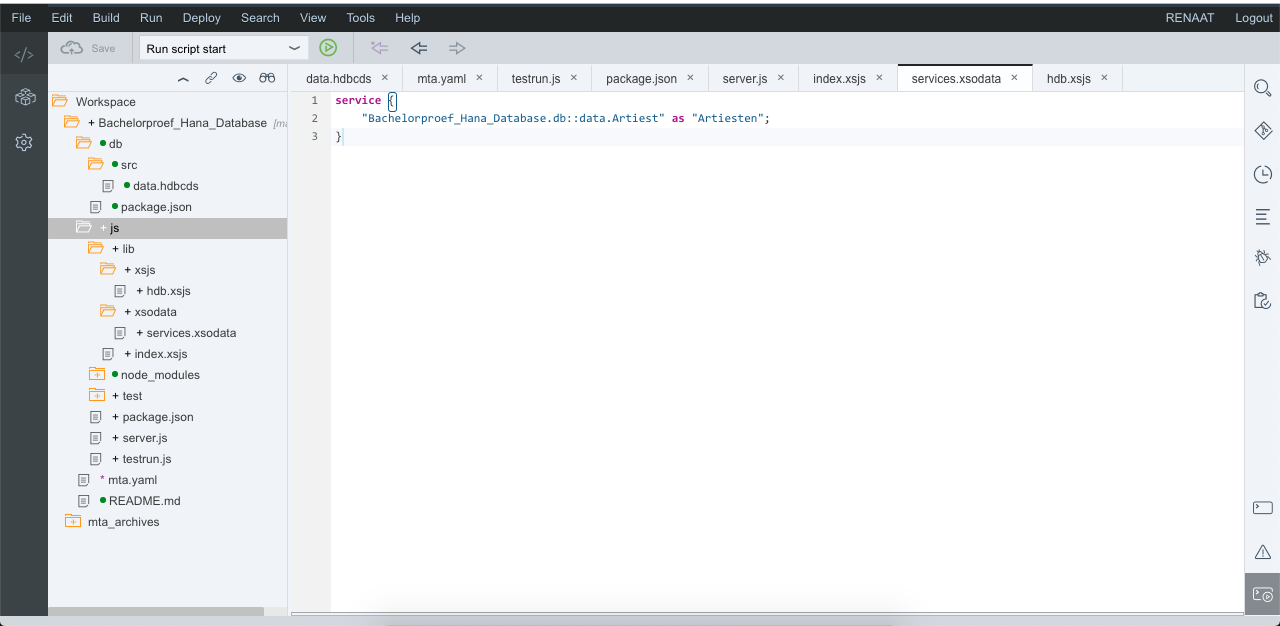
\includegraphics[scale=0.35]{HANA22}
                \caption{Opzetten HANA, stap 22} \label{HANA22}
            \end{figure}
            
            \begin{figure}	
                \centering
                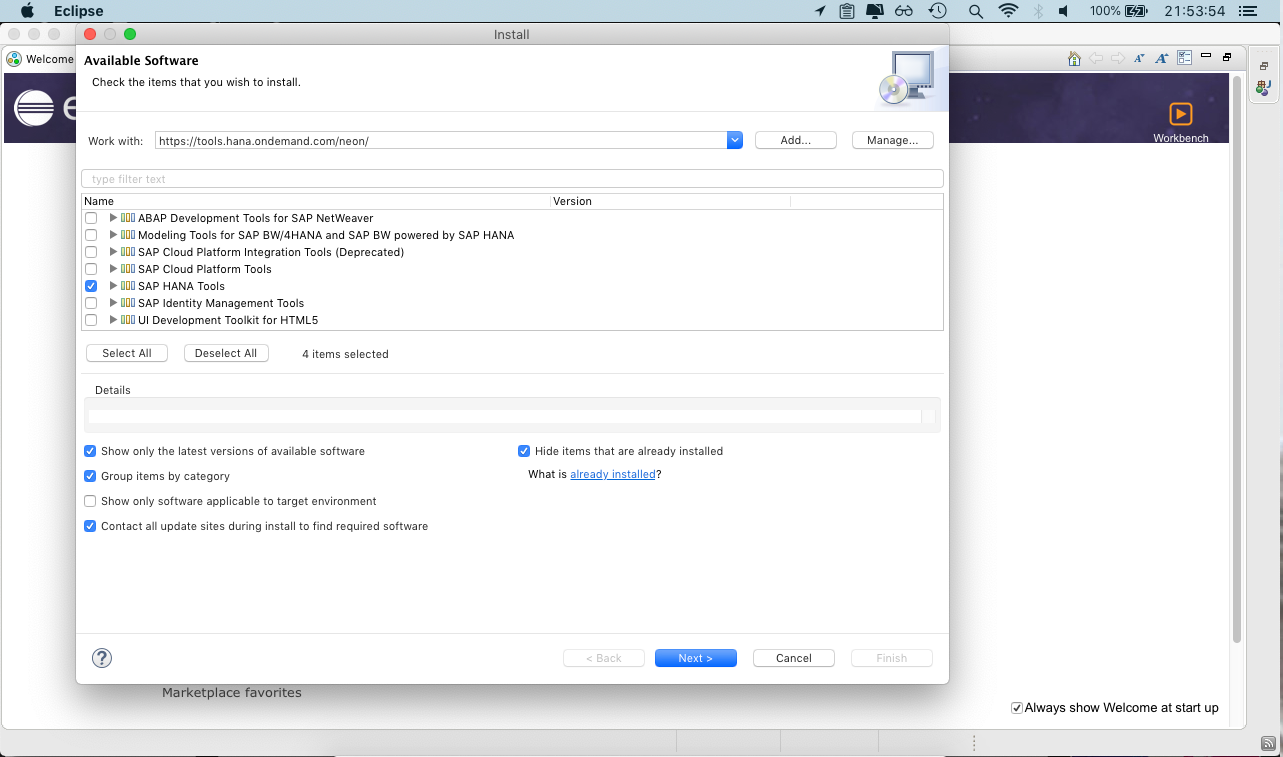
\includegraphics[scale=0.35]{HANA23}
                \caption{Opzetten HANA, stap 23} \label{HANA23}
            \end{figure}
           
            \paragraph{Node.js module}
            Om de models te gebruiken dat gecreëerd zijn, moeten we een tweede module toevoegen aan de HANA database: een Node.js module om de data als OData service te kunnen gebruiken.
            Deze module implementeert XSJS en XSODATA die op hun beurt zorgen voor de transformatie van het data model en de bereikbaarheid naar de buitenwereld. het is nodig om op de data CRUD (Create, Read, Update en Delete) operaties uit te voeren en als OData naar buiten gaat, dit is de taak van XSODATA. XSJS zorgt dan weer voor de integratie met SAPUI5. Het laat toe dat SAPUI5 applicaties de data kan lezen en kan bewerken.
            Zoals u in figuur \ref{HANA24} ziet moeten de instellingen aangepast worden. De feature Tools For Node.js Development moet beschikbaar zijn om te gebruiken in het project. Dit moet gesaved worden en het project moet opnieuw geladen worden. De volgende stap is de module maken door op het project met de rechtermuisknop te klikken, new en dan Node.js Module kiezen. Geef het een goede naam (js is good practice) en zorg ervoor dat Enable XSJX support aangevinkt is alvorens op Finish te klikken, zoals te zien is in figuur \ref{HANA25}, \ref{HANA26} en \ref{HANA27}.
            Databeveiliging is zeer belangrijk. Binnen HANA wordt er gebruik gemaakt van UAA (User Account en Authentication) om de Node.js module te beveiligen. Deze service moet samen met de database module en de HDI container, achter de db module, toegevoegd worden als resource zoals te zien valt in figuur \ref{HANA28}.
            Om een OData service te maken moeten volgende stappen gebeuren: in de js-module in de lib folder, moet een xsodata-file gemaakt worden in een nieuwe folder, xsodata genaamd. De link met de data moet in deze nieuwe file gemaakt worden. Later zal er ook de associatie moeten gemaakt worden tussen Artiest en Album. Deze stappen zijn te zien in figuren \ref{HANA29} en \ref{HANA30}.
            De volgende stap is de xsjs service maken door in de lib folder een nieuwe folder, xsjs genaamd, te maken met de nieuwe hdb.xsjs file. Zie figuur \ref{HANA31}. De inhoud van deze nieuwe file is te zien in figuur \ref{HANA32}.
            De nieuwe Node.js module moet gebuild worden door op de module met de rechtermuisknop te klikken, Run, Run As en dan Node.js Application te kiezen zoals te zien is in figuur \ref{HANA33}.
            Om de data uit de database te krijgen is het nodig om de url aan te passen. Het laatste na de poortnummer moet vervangen worden door: '/xsjs/hdb.xsjs'. Eens dit ingevoerd is, wordt de data in een Excel-bestand gedownload.
            \begin{figure}	
                \centering
                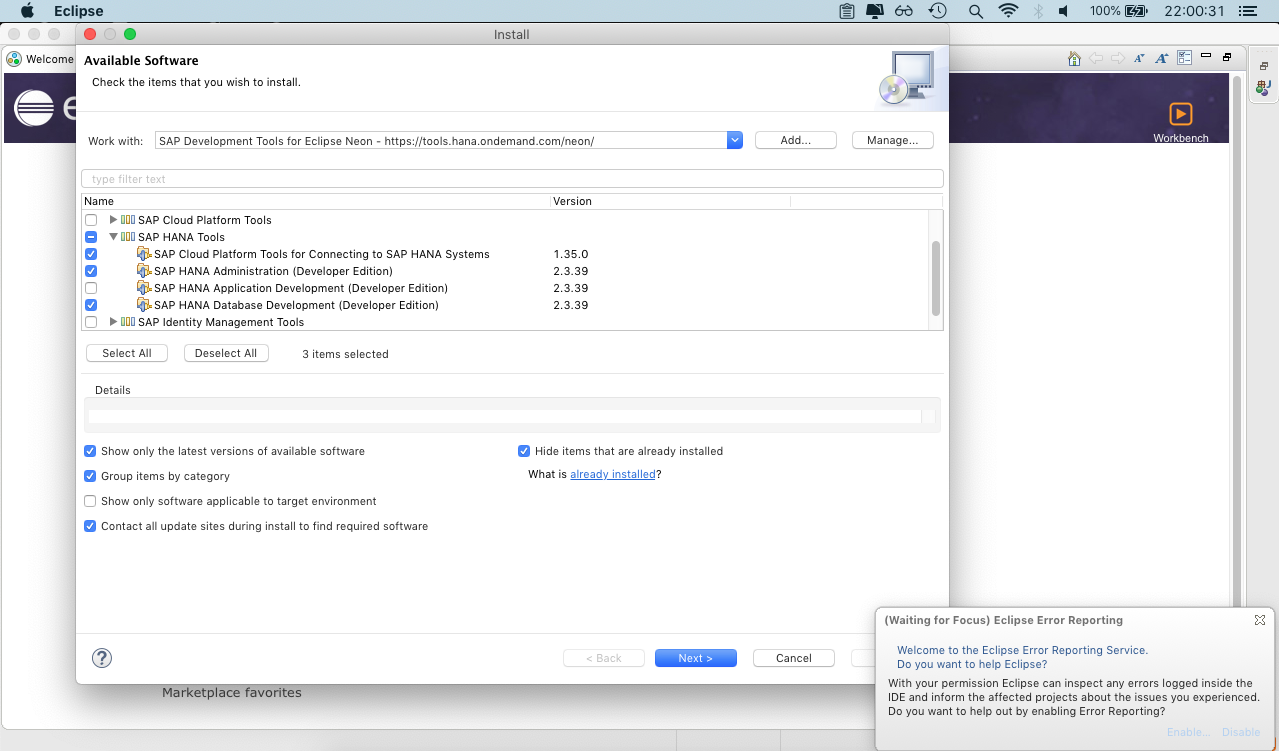
\includegraphics[scale=0.35]{HANA24}
                \caption{Opzetten HANA, stap 24} \label{HANA24}
            \end{figure}
            
            \begin{figure}	
                \centering
                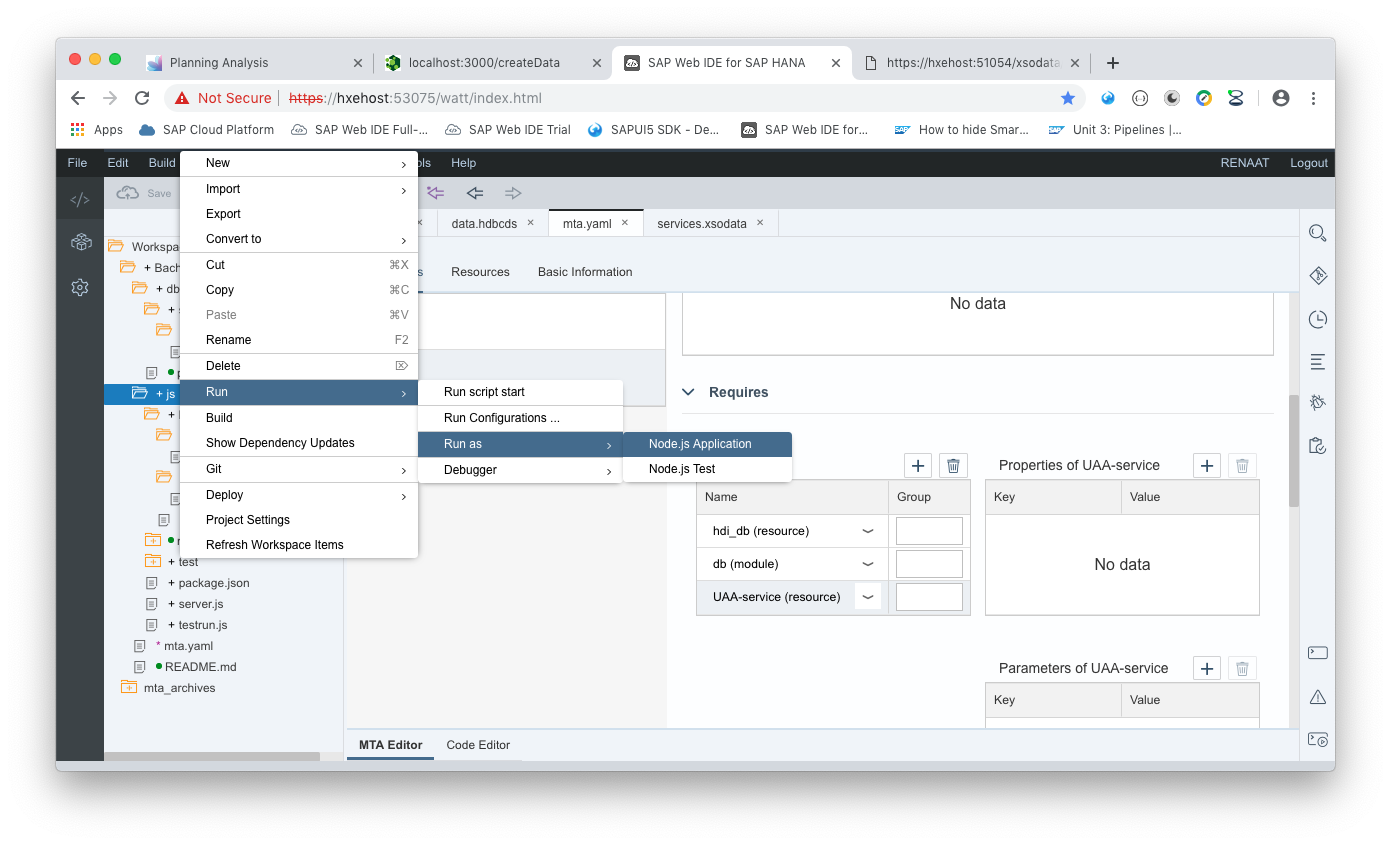
\includegraphics[scale=0.35]{HANA25}
                \caption{Opzetten HANA, stap 25} \label{HANA25}
            \end{figure}
            
            \begin{figure}	
                \centering
                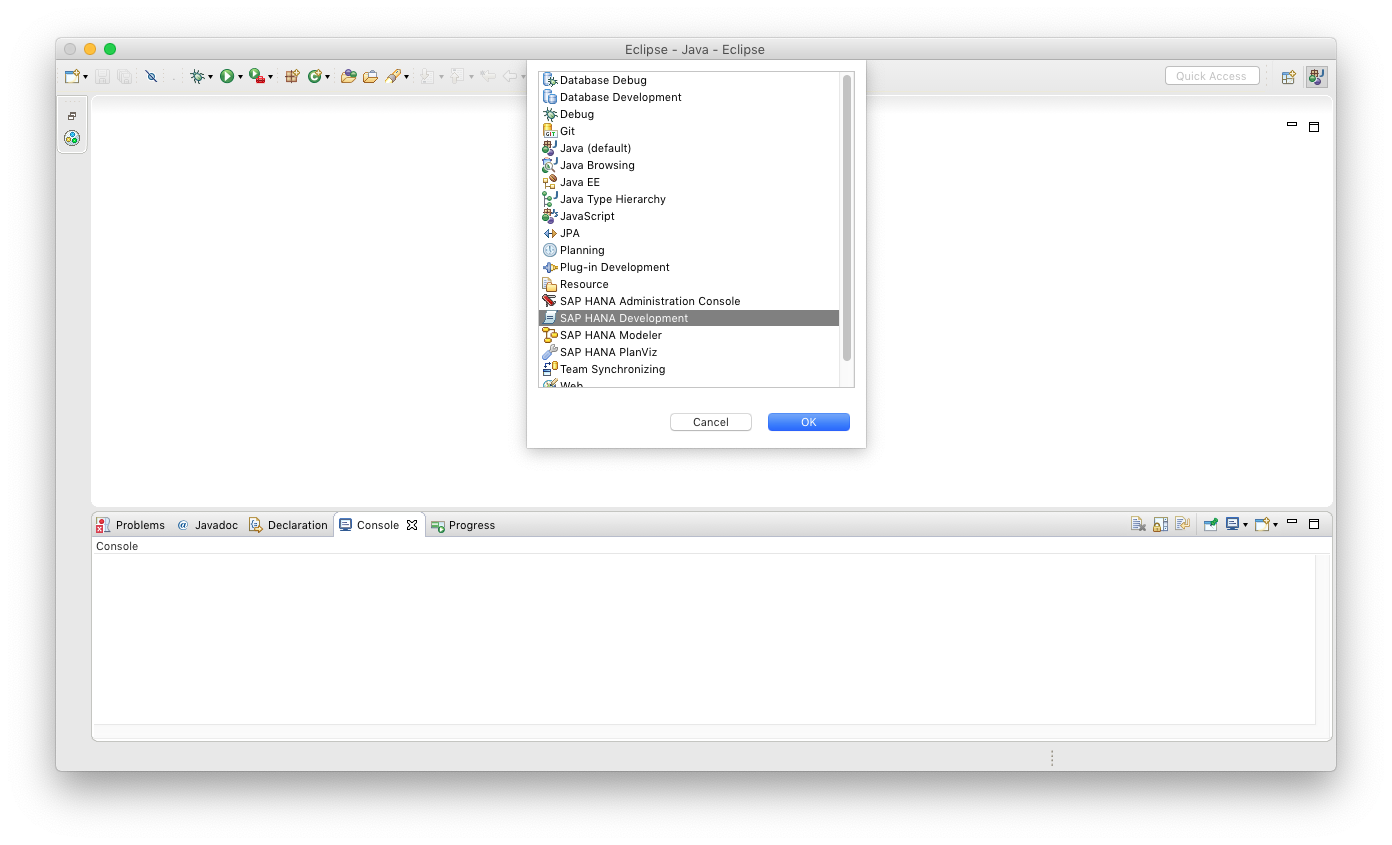
\includegraphics[scale=0.35]{HANA26}
                \caption{Opzetten HANA, stap 26} \label{HANA26}
            \end{figure}
            
            \begin{figure}	
                \centering
                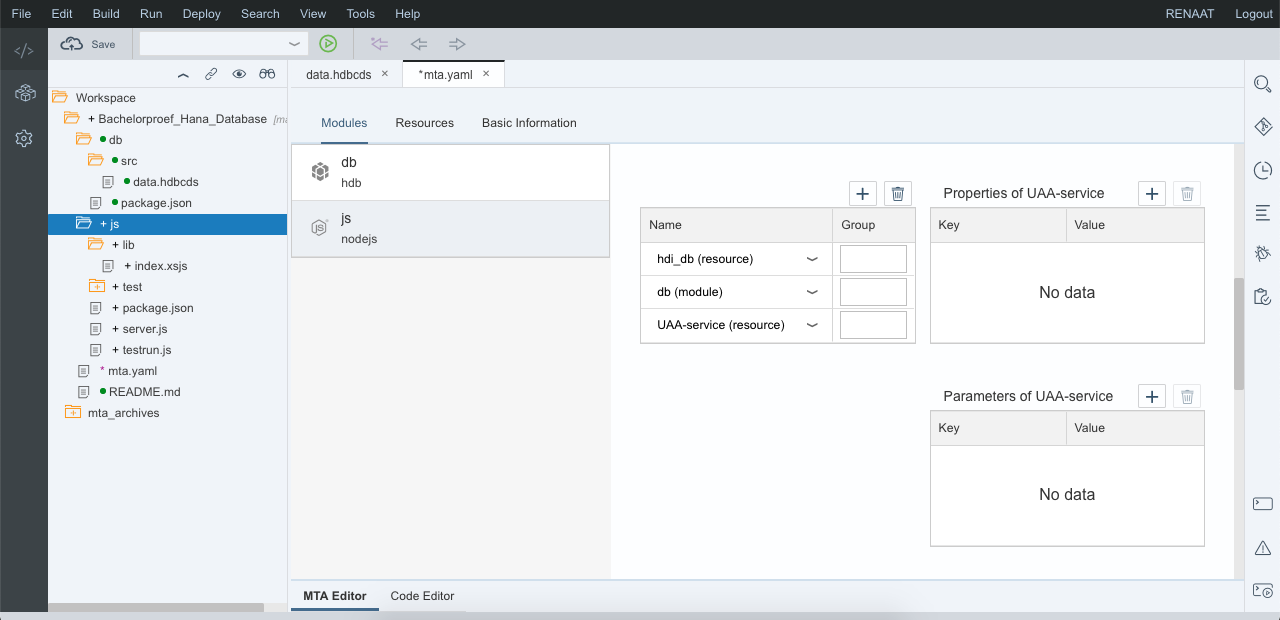
\includegraphics[scale=0.35]{HANA27}
                \caption{Opzetten HANA, stap 27} \label{HANA27}
            \end{figure}
            
            \begin{figure}	
                \centering
                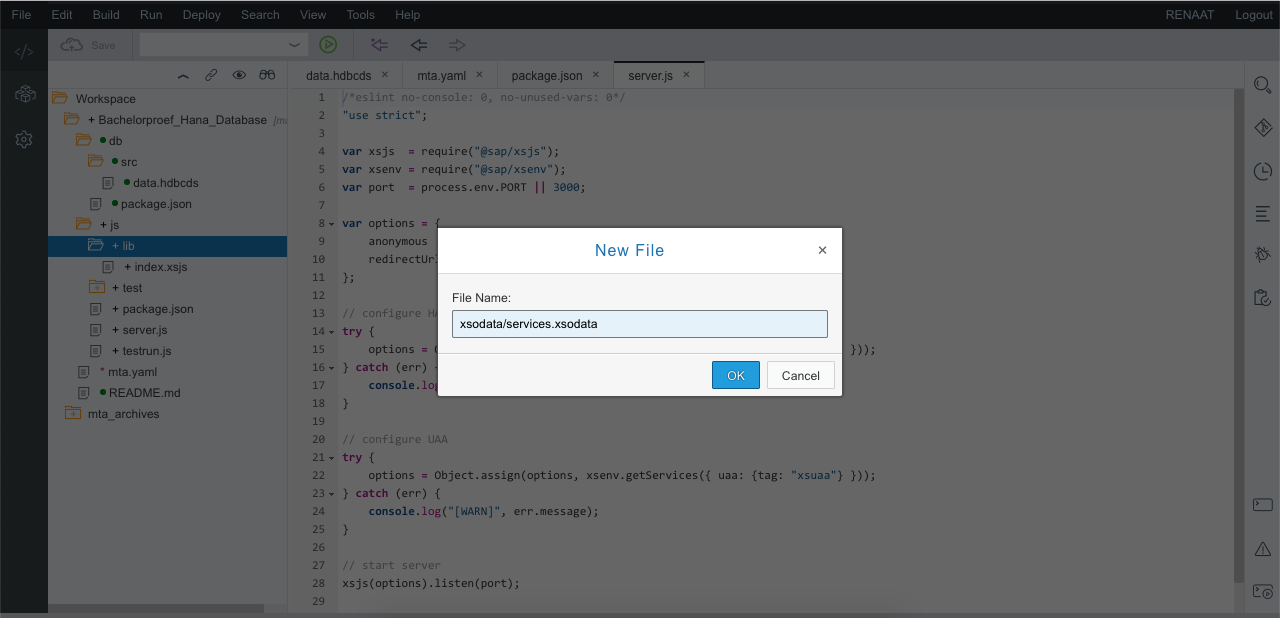
\includegraphics[scale=0.35]{HANA28}
                \caption{Opzetten HANA, stap 28} \label{HANA28}
            \end{figure}
            
            \begin{figure}	
                \centering
                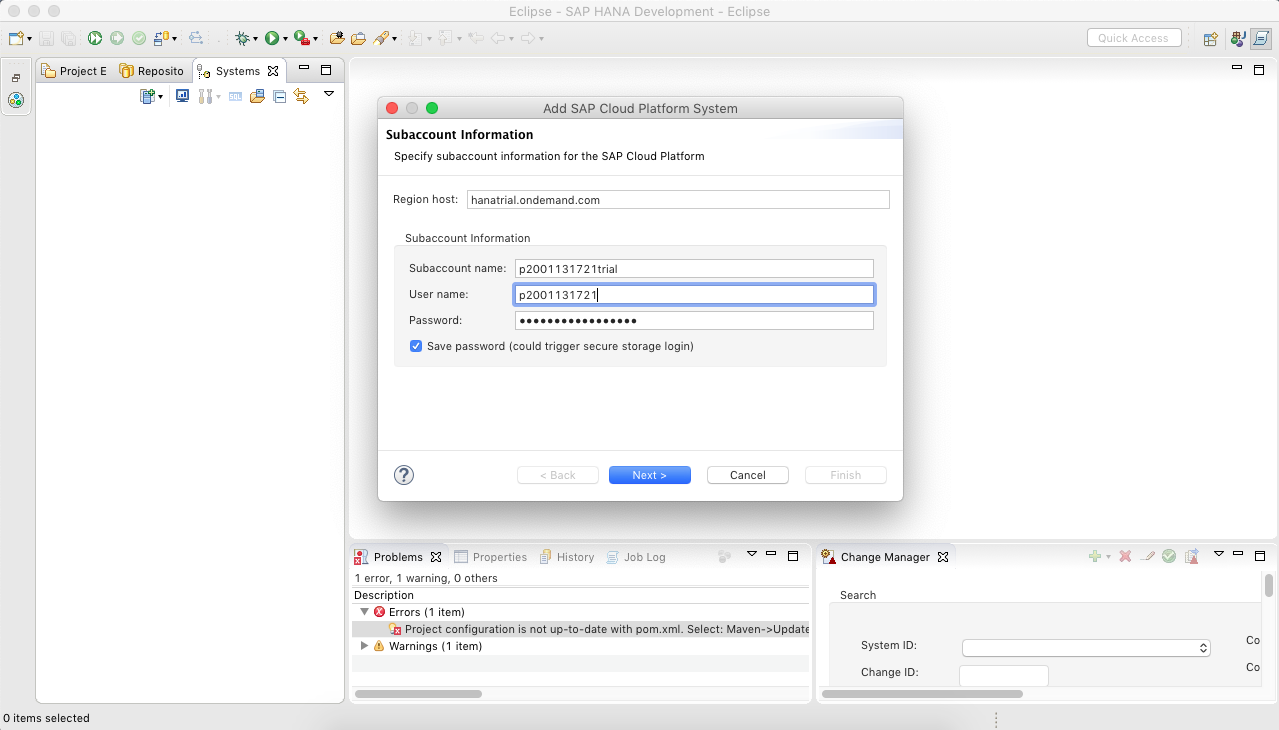
\includegraphics[scale=0.35]{HANA29}
                \caption{Opzetten HANA, stap 29} \label{HANA29}
            \end{figure}
        
            \begin{figure}	
                \centering
                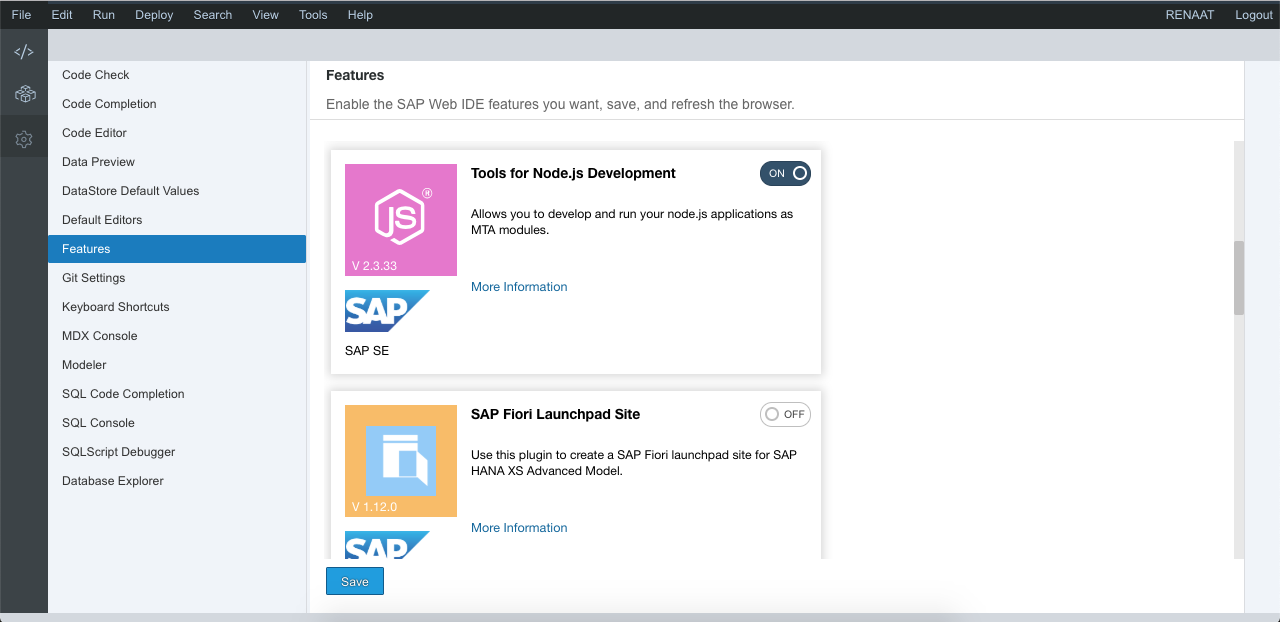
\includegraphics[scale=0.35]{HANA30}
                \caption{Opzetten HANA, stap 30} \label{HANA30}
            \end{figure}
            
            \begin{figure}	
                \centering
                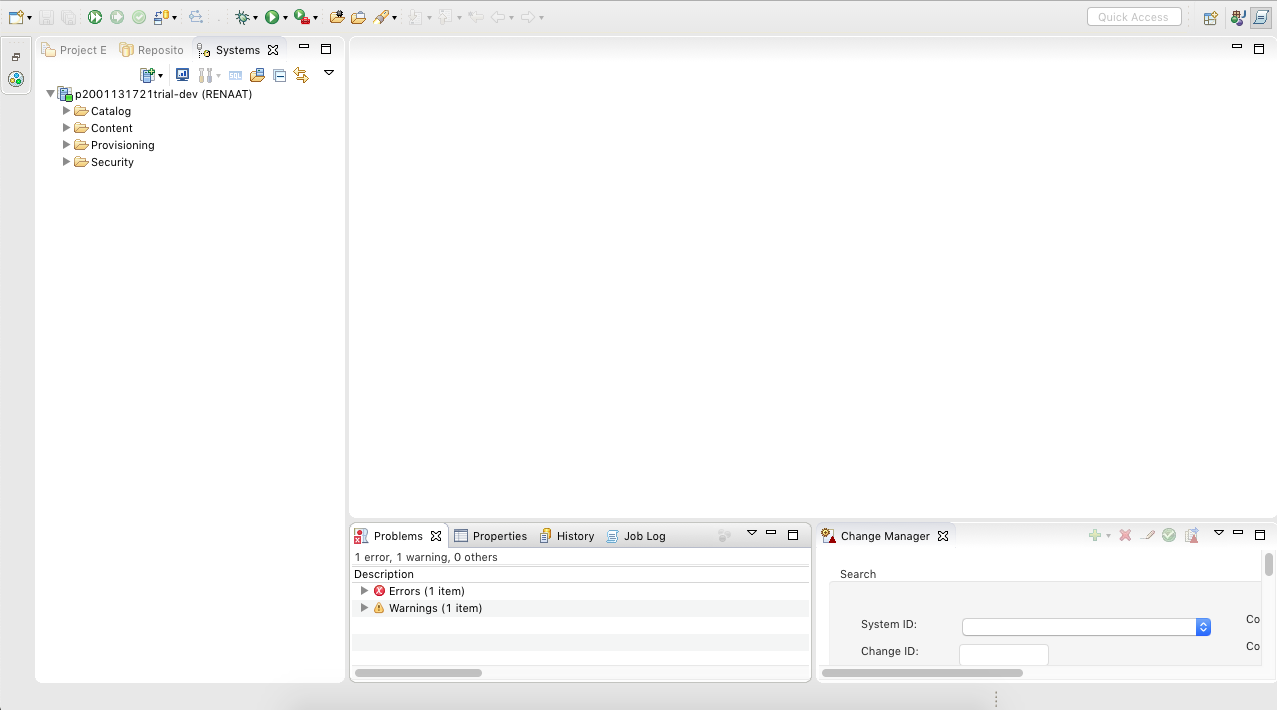
\includegraphics[scale=0.35]{HANA31}
                \caption{Opzetten HANA, stap 31} \label{HANA31}
            \end{figure}
            
            \begin{figure}	
                \centering
                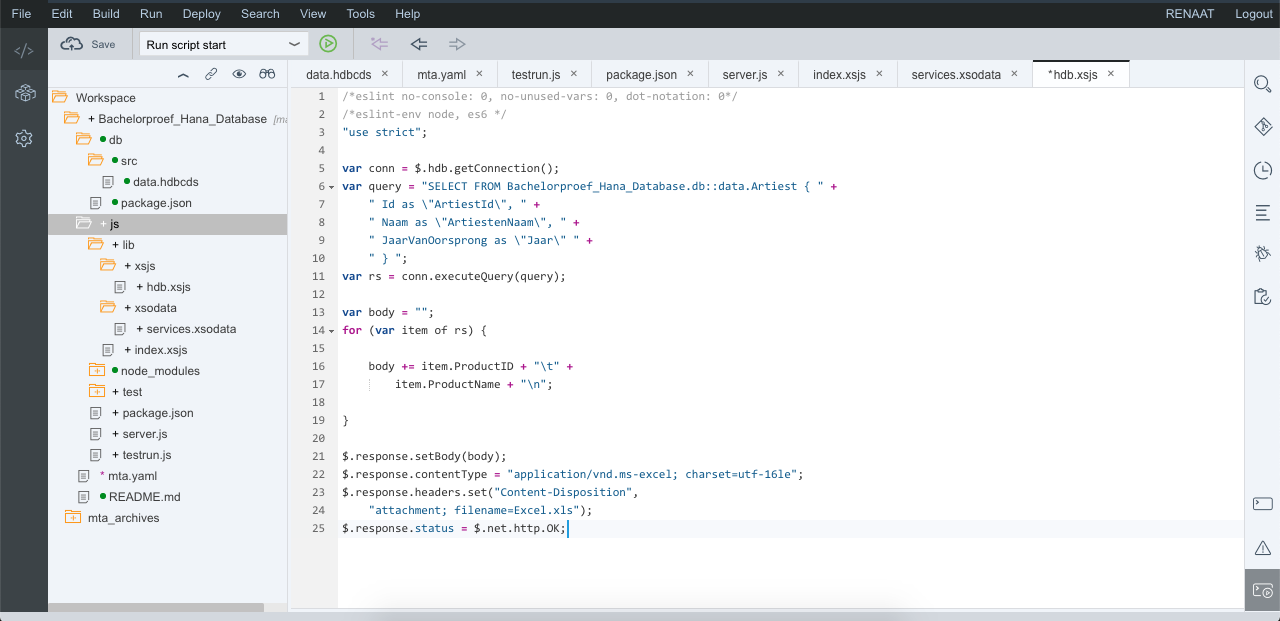
\includegraphics[scale=0.35]{HANA32}
                \caption{Opzetten HANA, stap 32} \label{HANA32}
            \end{figure}
            
            \begin{figure}	
                \centering
                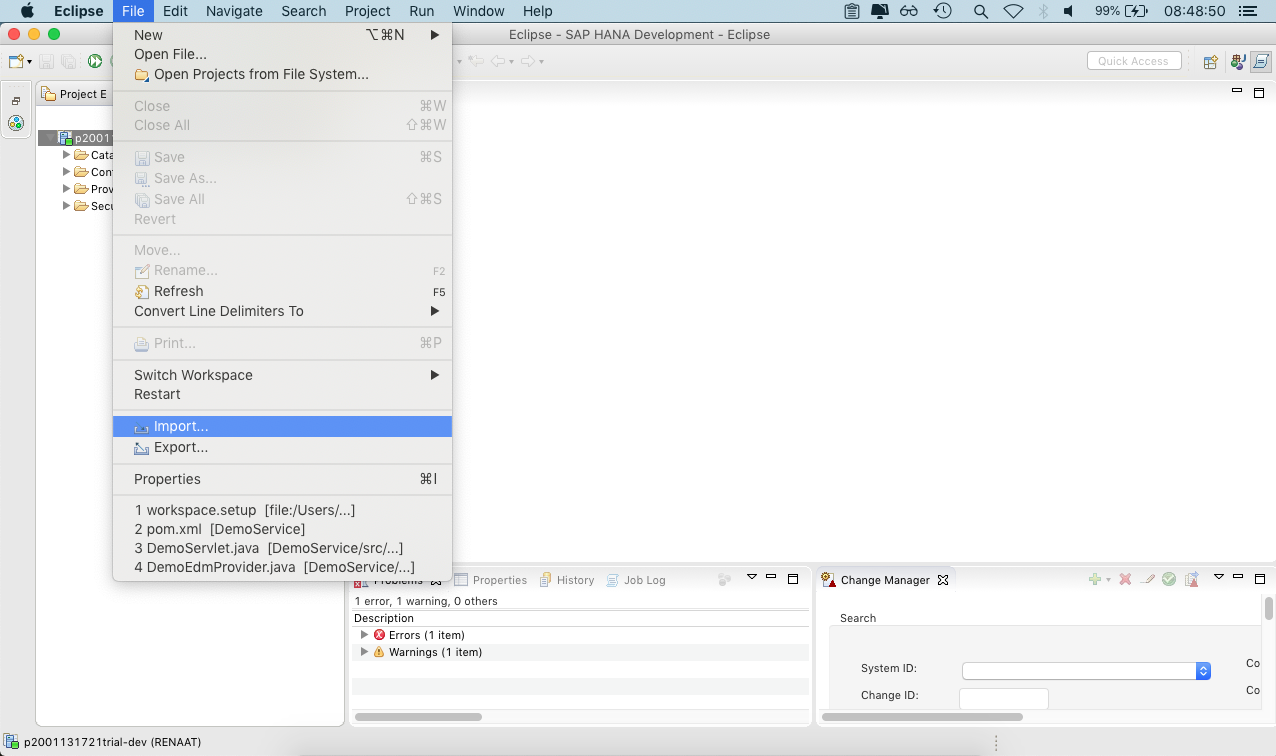
\includegraphics[scale=0.35]{HANA33}
                \caption{Opzetten HANA, stap 33} \label{HANA33}
            \end{figure} 
            
        \subsection{Automated testing binnen SAPUI5}
        \label{subsec:automated-testing-SAPUI5}
        %TODO: https://help.sap.com/viewer/468a97775123488ab3345a0c48cadd8f/7.52.1/en-US/ae448243822448d8ba04b4784f4b09a0.html
        %TODO: https://blogs.sap.com/2016/11/21/headless-opa5-testing-with-karma-and-phantomjs/